% vim: tw=80

\chapter{Constraints on PDFs and Determination of the Strong Coupling Constant}
\label{sec:pdf_constraints}

In many precision measurements at the LHC, the proton PDFs are an essential
ingredient. Since the PDFs cannot be calculated from perturbative QCD, they are
determined in fits to experimental data of collider and fixed-target experiments.
The precise DIS data from the combined measurements of the HERA-I and HERA-II
run periods\footnote{In the following, the combined HERA-I and HERA-II DIS data sets
are always referred to as HERA DIS data.} provides the base data set since it
covers a large part of the kinematic phase space. By including more data from different
experiments which provide constraints in additional phase space regions, the
precision on the PDFs can be improved. In a similar way, the impact of the
triple-differential dijet cross section on the PDFs are studied by performing a
fit of the combined HERA DIS data and the triple-differential dijet cross
section measurement.

As discussed in Sec.~\ref{sec:nlo_comparisons}, the electroweak corrections have
not been available in time for this thesis. They are large only at highest
transverse momenta and central rapiditities. Thus, the bins with $\ptavg >
\SI{1000}{\GeV}$ have not been considered in the PDF studies removing 11 of 144
bins.  However, the experimental uncertainties of the neglected bins is
comparably large, hence their impact on the fit result is small.

\section{Correlation between Dijet Cross Section and PDFs}
\label{sec:pdf_sensitivity}

To illustrate the phase space regions in which the triple-differential dijet
cross section measurement has an impact on the PDFs, the correlation between the cross
section $\sigma(\mu)$ and the PDFs $xf(x,\mu^2)$ for any parton flavor~$f$ can be
calculated. The PDF sets of the NNPDF collaboration are an ensemble of replicas
$i$, which sample variations in the PDF parameter space within the PDF's
uncertainties. The correlation coefficient $\varrho_f(x,\mu)$ between the cross
section and the PDF for flavor~$f$ at a point $(x,\mu)$ can be calculated by
evaluating the mean and standard deviation from an ensemble of $N$ replicas as

\begin{equation}
  \varrho_f (x,\mu) =
  \frac{N}{(N-1)} \frac{%
    \langle \sigma(\mu)_i \cdot xf(x,\mu^2)_i \rangle -
    \langle \sigma(\mu)_i \rangle \cdot
    \langle xf(x,\mu^2)_i \rangle}
  {\Delta_{\sigma(\mu)} \Delta_{xf(x,\mu^2)}}\,.
\end{equation}

where $\Delta_{\sigma(Q)}$ and $\Delta_{xf(x,Q^2)}$ are the standard deviations of the
dijet cross section and of the PDF with flavor $f$, respectively.
Fig.~\ref{fig:correlation_pdf_xs_gqq} presents the correlation coefficient
between the dijet cross section and the gluon, u valence quark, and d valence
quark PDFs for the central region ($\yboost < 1, \ystar < 1$) and the
boosted region ($2 \leq \yboost < 3$).

\begin{figure}[p]
  \centering
  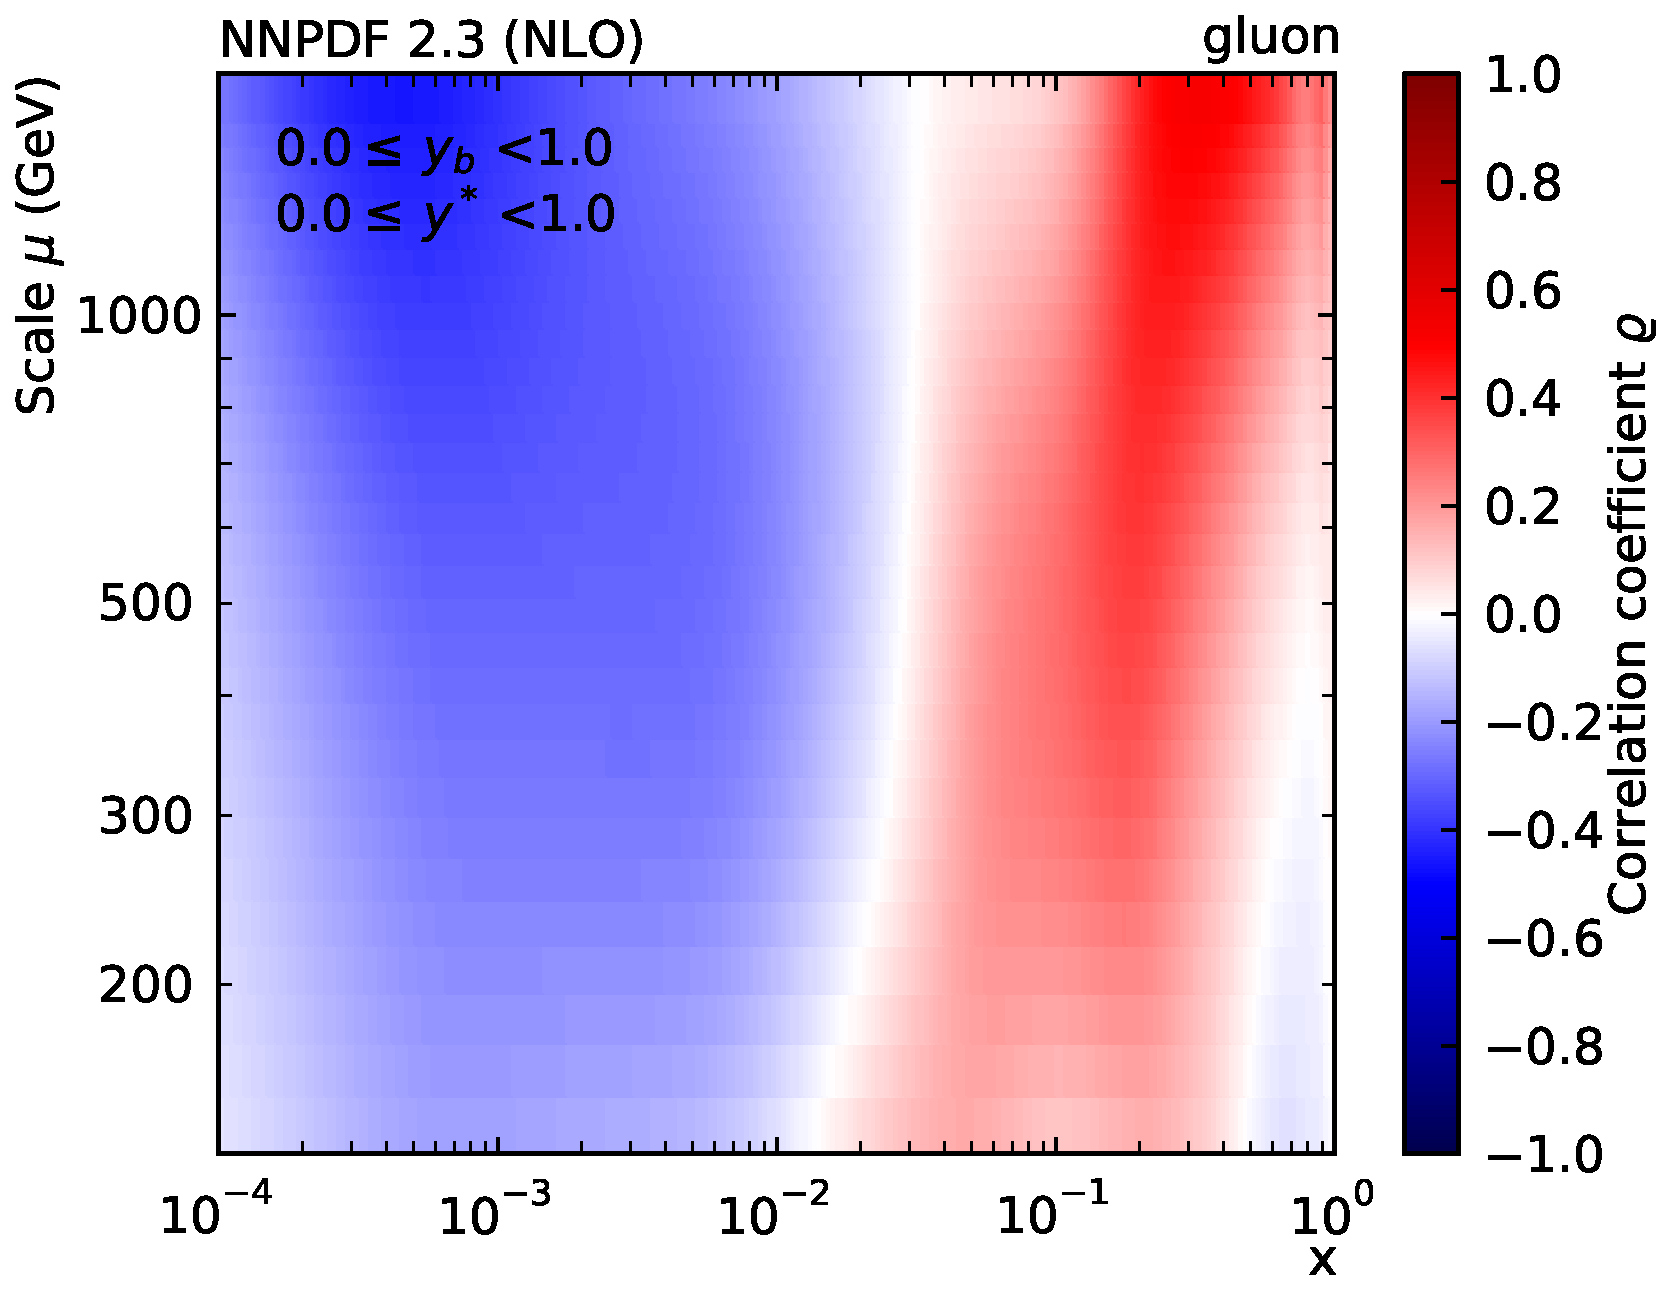
\includegraphics[width=0.49\textwidth]{figures/pdf_constraints/corr_PTMAXEXPYS_YBYS_NLO_FINALBINS_NNPDF23_gluon_ys0_0yb0_0_cl.pdf}\hfill%
  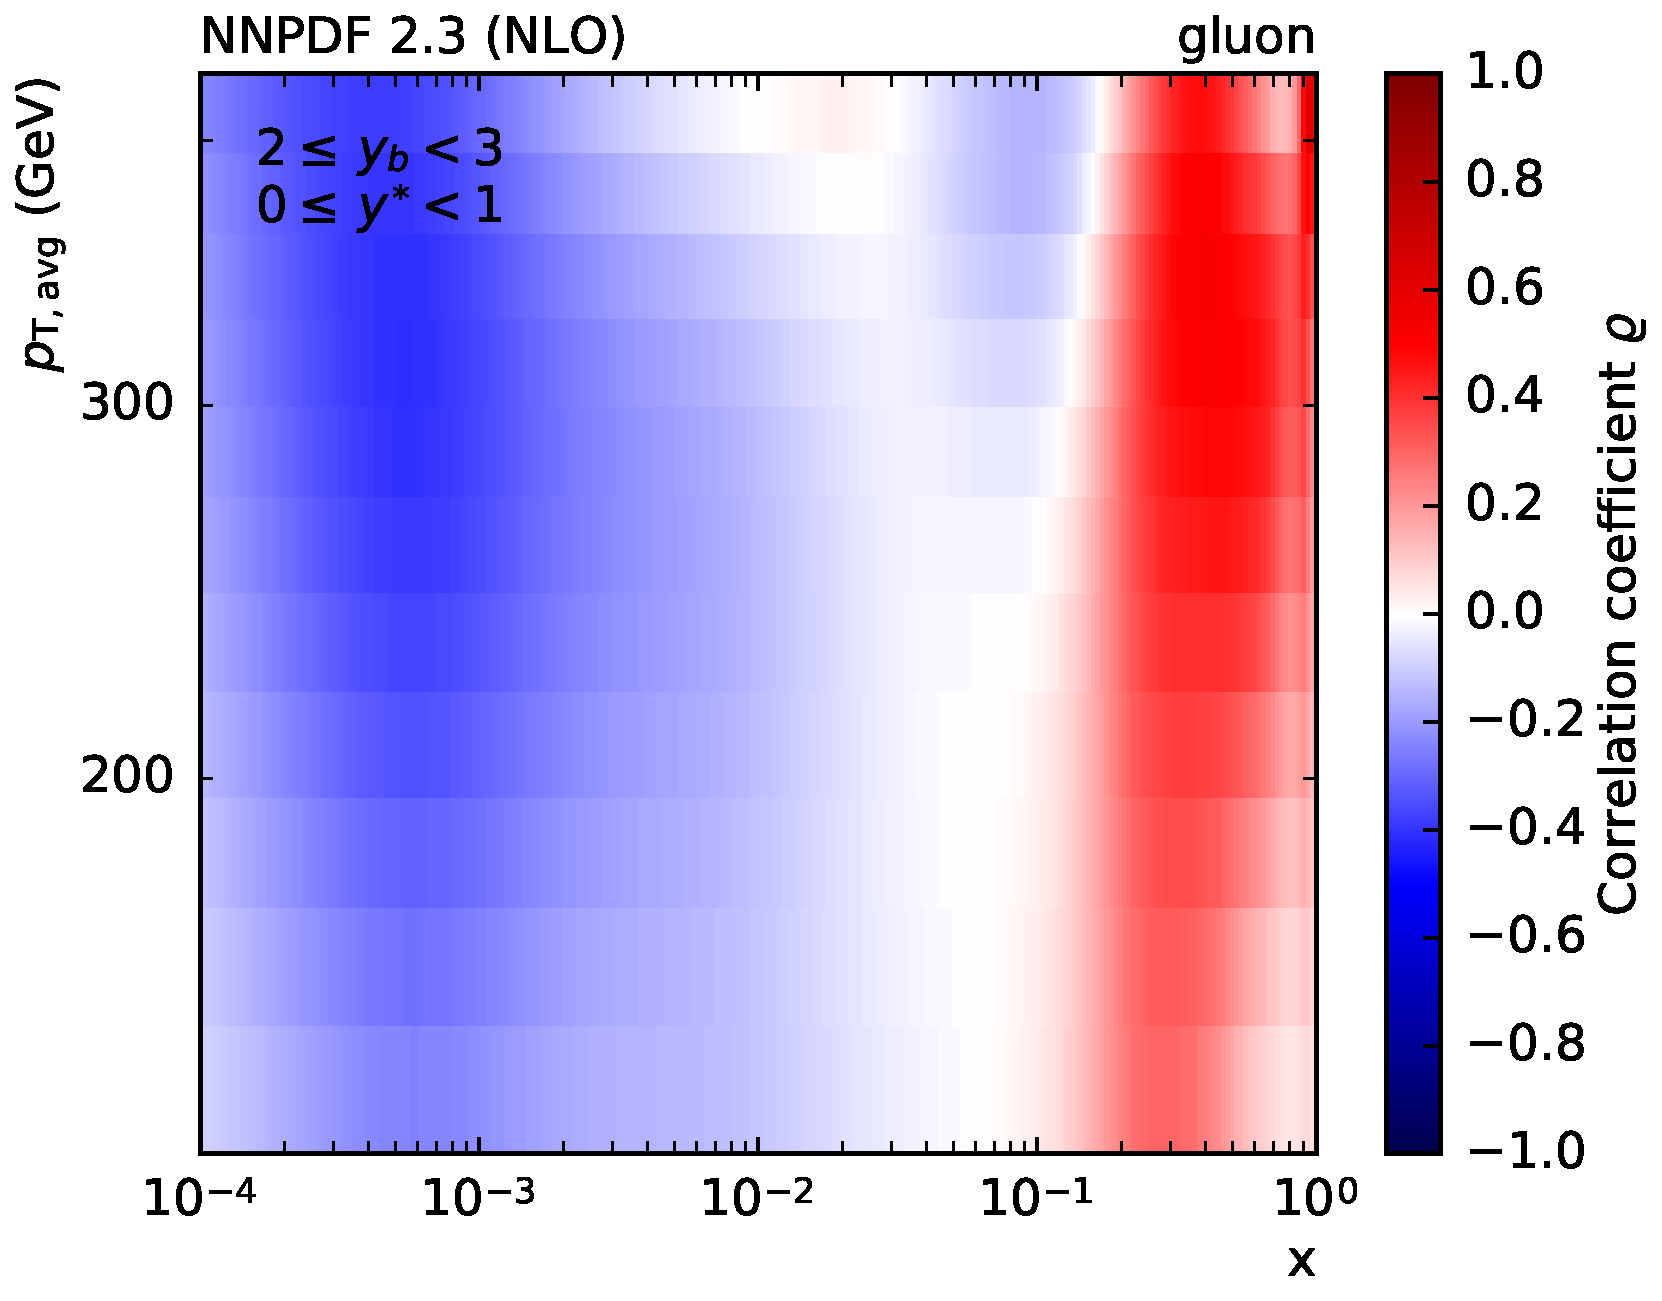
\includegraphics[width=0.49\textwidth]{figures/pdf_constraints/corr_PTMAXEXPYS_YBYS_NLO_FINALBINS_NNPDF23_gluon_ys0_0yb2_0_cl.pdf}
  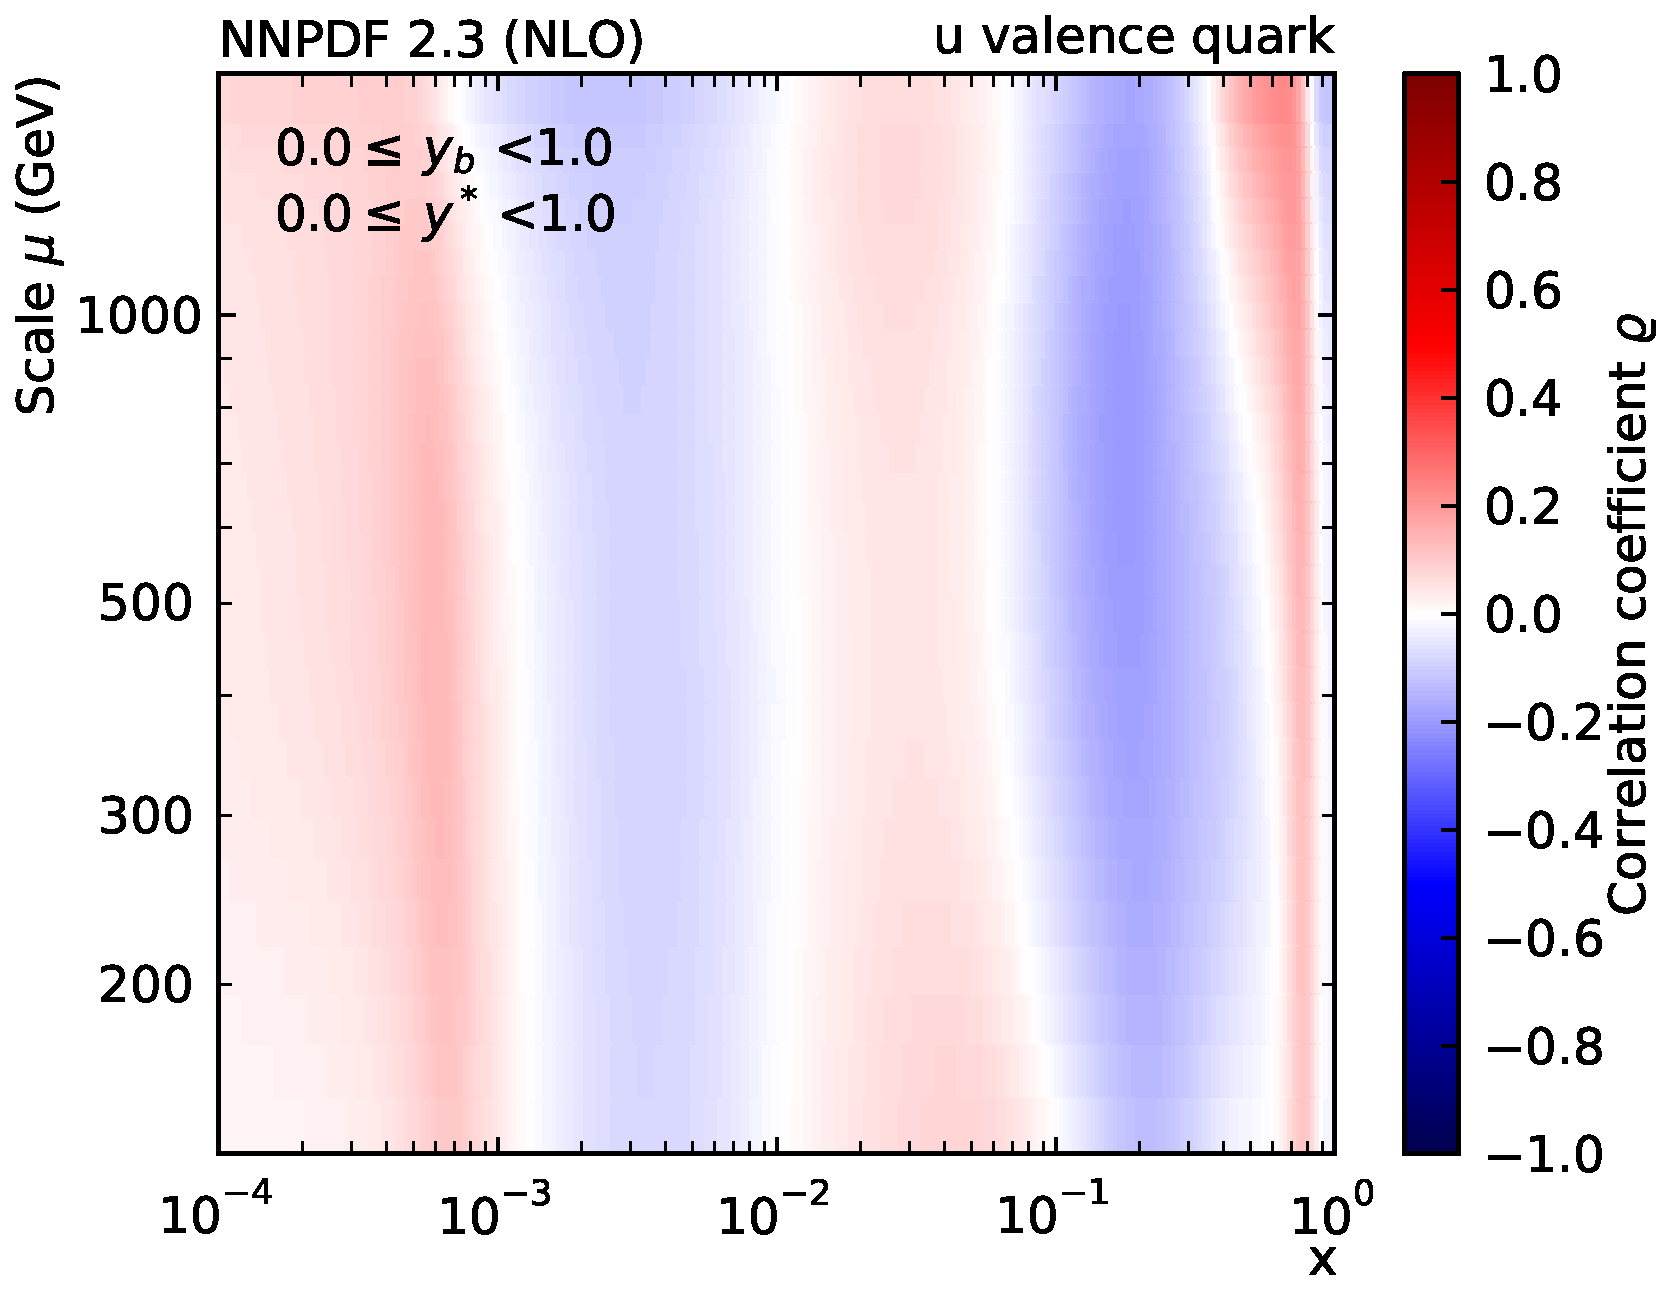
\includegraphics[width=0.49\textwidth]{figures/pdf_constraints/corr_PTMAXEXPYS_YBYS_NLO_FINALBINS_NNPDF23_u_valence_quark_ys0_0yb0_0_cl.pdf}\hfill%
  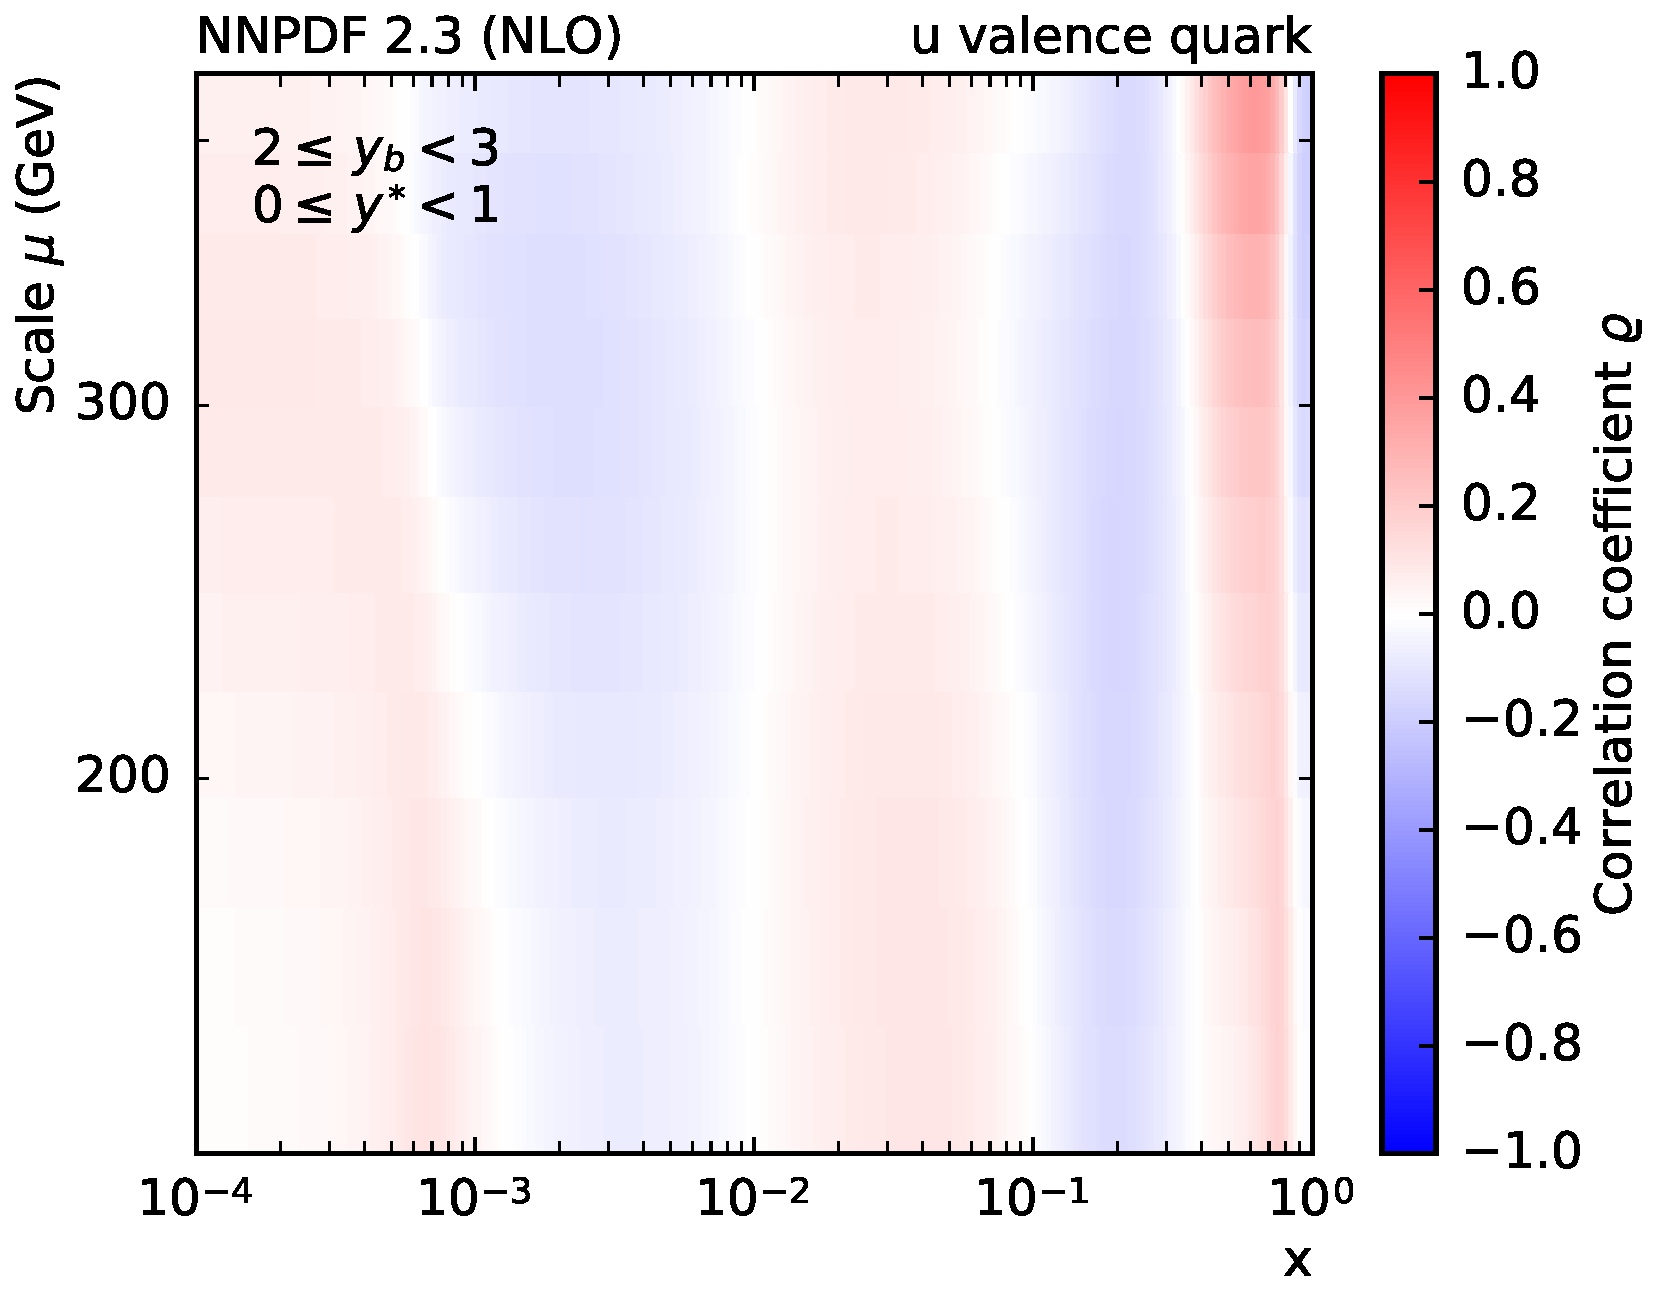
\includegraphics[width=0.49\textwidth]{figures/pdf_constraints/corr_PTMAXEXPYS_YBYS_NLO_FINALBINS_NNPDF23_u_valence_quark_ys0_0yb2_0_cl.pdf}
  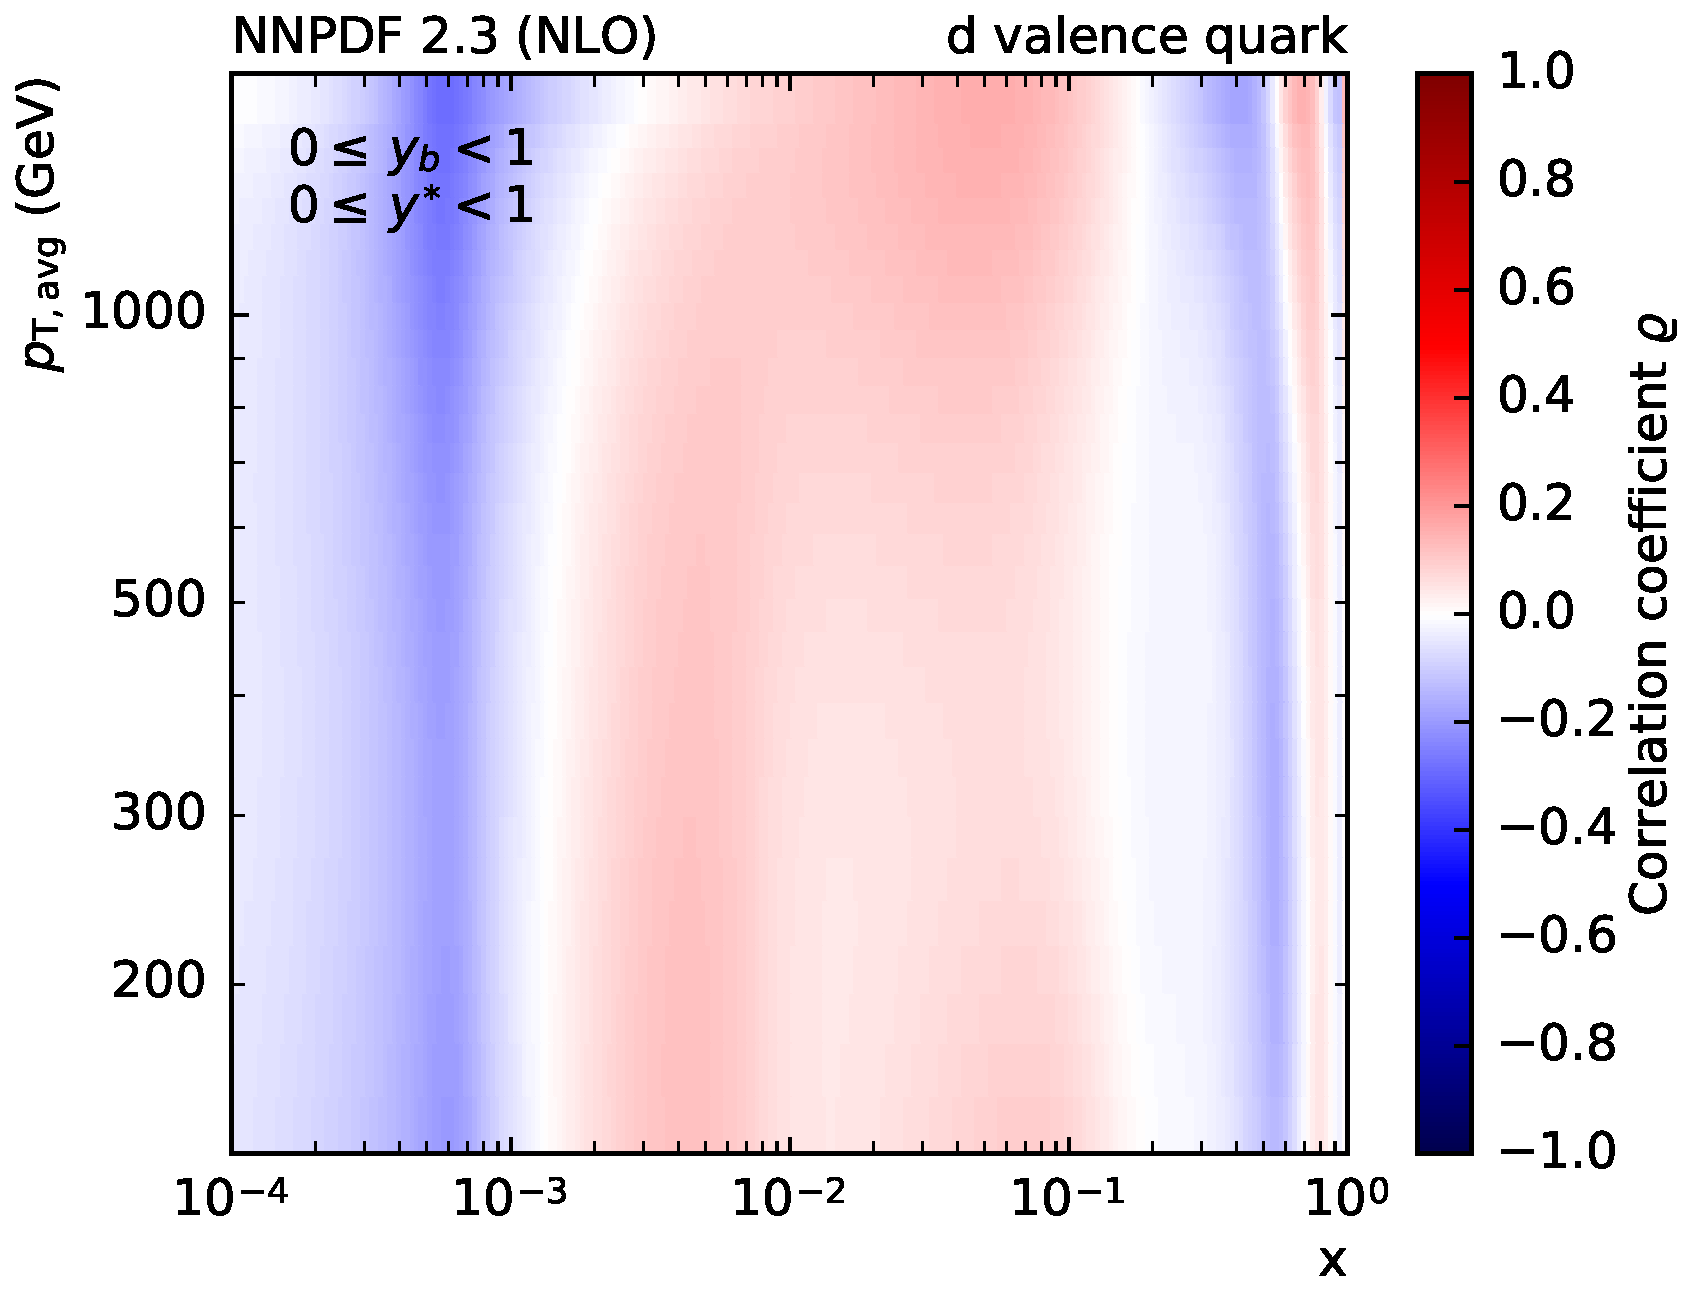
\includegraphics[width=0.49\textwidth]{figures/pdf_constraints/corr_PTMAXEXPYS_YBYS_NLO_FINALBINS_NNPDF23_d_valence_quark_ys0_0yb0_0_cl.pdf}\hfill%
  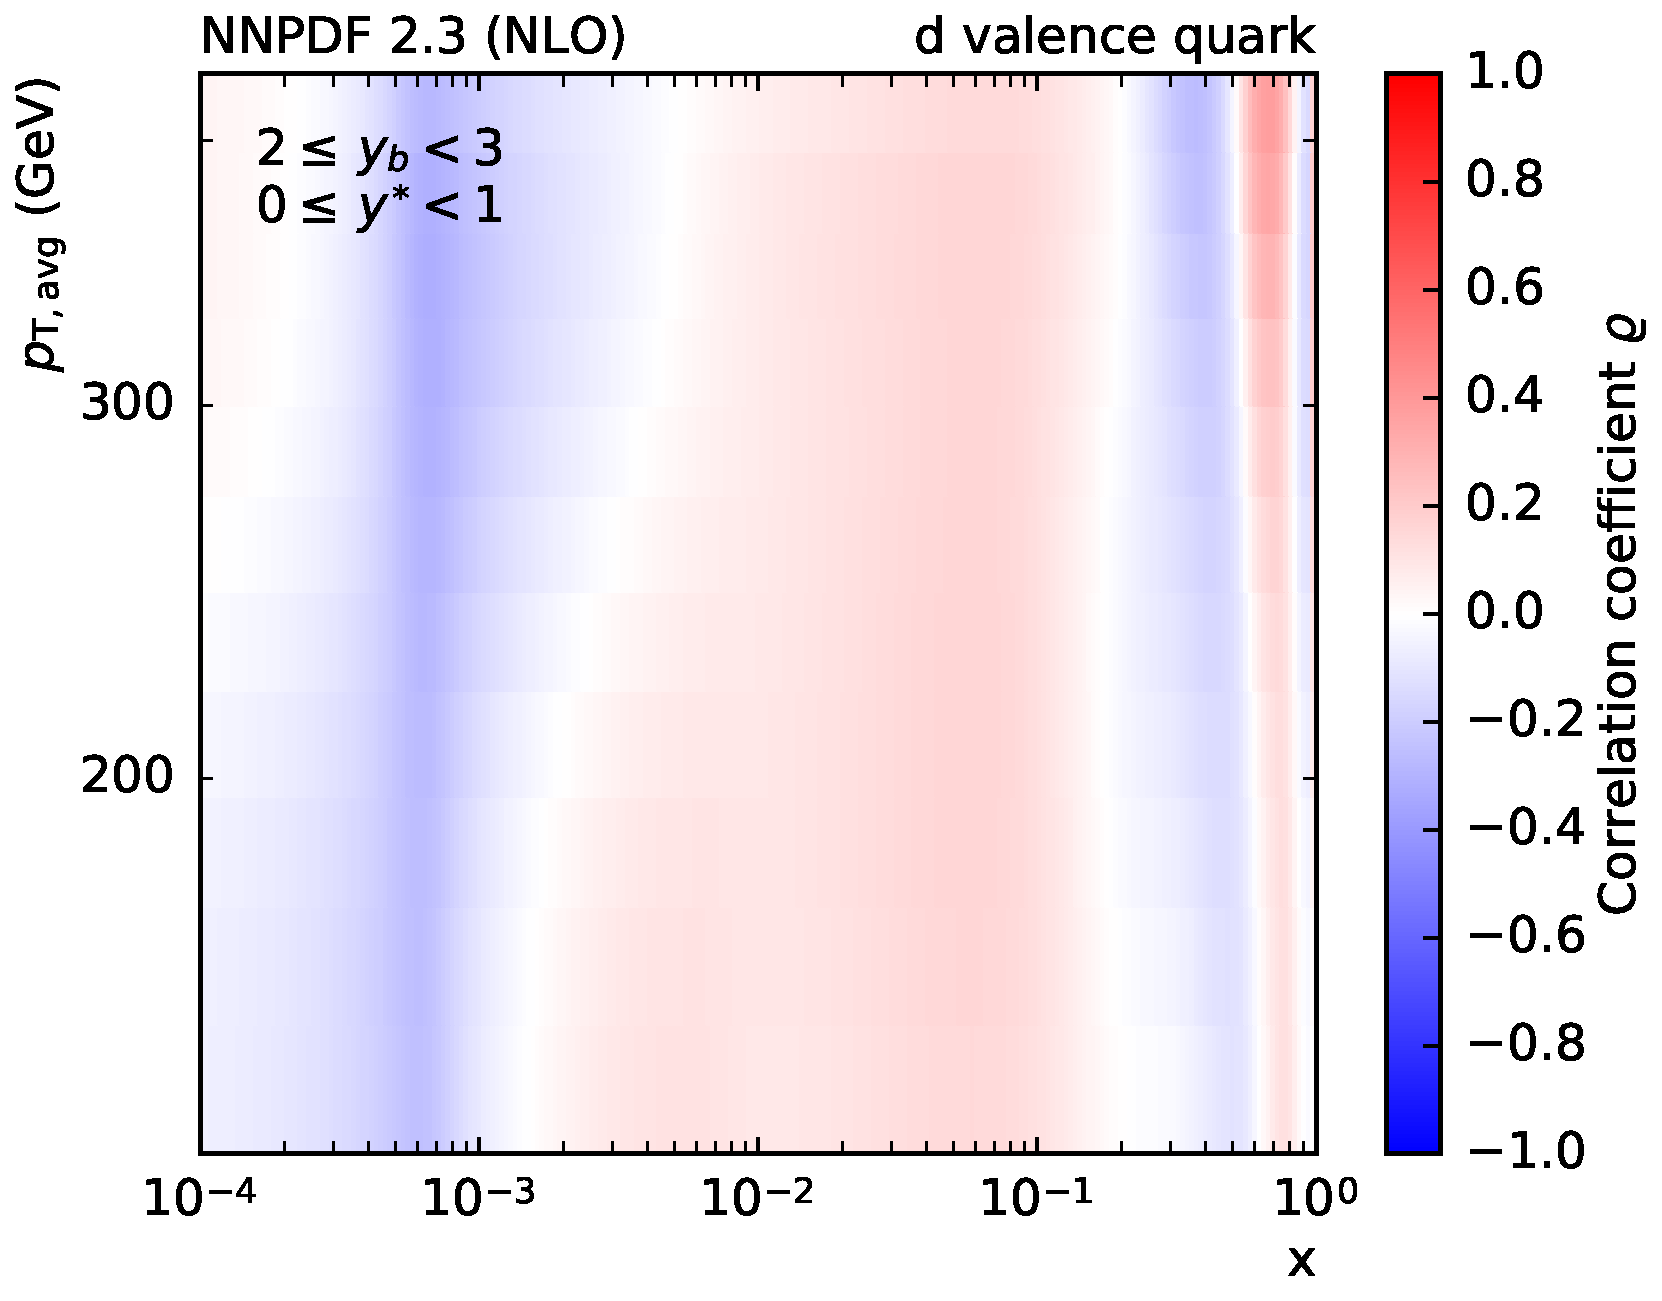
\includegraphics[width=0.49\textwidth]{figures/pdf_constraints/corr_PTMAXEXPYS_YBYS_NLO_FINALBINS_NNPDF23_d_valence_quark_ys0_0yb2_0_cl.pdf}
  \caption[Correlation between dijet cross section and PDFs]{
    The correlation coefficient between the triple-differential dijet cross
    section and the gluon (top row), the u valence quark (middle row),
    and the d valence quark PDFs (bottom row) as a function of the
    momentum fraction $x$ of the proton and the energy scale $\mu$ of
    the hard process. The correlation is shown for the central
    bin $\yboost < 1,\,\ystar < 1$ (left) and for the boosted region $2 \leq
    \yboost < 3$ (right).}
  \label{fig:correlation_pdf_xs_gqq}
\end{figure}

The correlation between the gluon PDF and the dijet cross section is large in
the central bin for \ptavg > \SI{1}{\TeV} and momentum fractions $0.1 < x <
0.5$. In the boosted region there is a large correlation for $\SI{200}{\GeV}
\leq \ptavg < \SI{400}{\GeV}$ and momentum fractions $0.2 < x < 0.7$. In
contrast, the correlation between the dijet cross section and the u valence and
d valence quark PDFs is much smaller, especially in the central region. However,
the correlation in the boosted region is more pronounced, particularly for
highest momentum fractions $x > 0.5$. Additional figures with the correlations
of the others bins can be found in the appendix in the
Figs.~\ref{fig:pdfconstraints_gluon}--\ref{fig:pdfconstraints_sea_quarks}. Based
on the results of the correlation studies, a significant impact of the dijet
cross section is expected by including the dijet cross sections in a PDF fit.

\section{The \xfitter Framework}
\label{section:herafittersetup}

The constraints of the triple-differential dijet measurement on the proton PDFs
are demonstrated by including the cross section measurement in a PDF fit in
combination with inclusive DIS cross sections from the HERA experiments. The
combined HERA-I and HERA-II DIS data were the
basis for the determination of the HERAPDF 2.0 PDF set.

\xfitter~\cite{Alekhin:2014irh} is an open source framework to fit the PDFs to experimental data based
on the DGLAP~\cite{Gribov:1972ri,Altarelli:1977zs,Dokshitzer:1977sg} equations.
To ensure consistency between DIS and QCD calculations, the fits are performed
at NLO as the latter are only available at that order. The DIS cross sections
are calculated by the QCDNUM software~\cite{Botje:2010ay}.

The parametrization used in the PDF fit is based on the parametrization used for
the HERAPDF~2.0 determination~\cite{Abramowicz:2015mha}. After including the
dijet data, a study of the parametrization was performed resulting in a slightly
different parametrization found to better describe the included dijet data. The
most notable difference is the neglection of the negative gluon term. No
improvement of the fit result was found when including it. This is probably due
to minimum $Q^2$ cut imposed on the DIS data, which was adapted from
$Q^2_\mathrm{min}=\SI{3.5}{\GeVsq}$ to $Q^2_\mathrm{min}=\SI{7.5}{\GeVsq}$.
However, this additional negative gluon term was considered when deriving the
PDF parametrization uncertainties.

The parametrization of the PDFs is defined at the starting scale
$Q_0^2$ which is set to $Q_0^2 = \SI{1.9}{\GeV \squared}$ and the five
independent PDFs $xu_v(x)$, $xd_v(x)$, $xg(x)$, $x\bar{U}(x)$ and $x\bar{D}(x)$
are parametrized as follows:
%
\begin{align*}
  xg(x) &= A_g x^{B_g} (1-x)^{C_g} (1 + E_g x^2)\\
  xu_v(x) &= A_{u_{v}} x^{B_{u_{v}}} (1-x)^{C_{u_{v}}}(1 + D_{u_{v}}x)\\
  xd_v(x) &= A_{d_v} x^{B_{d_v}} (1-x)^{C_{d_{v}}}\\
  x\bar U(x) &= A_{\bar U} x^{B_{\bar U}} (1-x)^{C_{\bar U}}(1 + D_{\bar U}x)\\
  x\bar D(x) &= A_{\bar D} x^{B_{\bar D}} (1-x)^{C_{\bar D}}
\end{align*}
%
Actually, not all parameters are fitted. The normalization parameters $A_g$,
$A_{u_{v}}$ and $A_{d_{v}}$ are calculated using the QCD sum rules. $B_{\bar
U}=B_{\bar D}$ and $A_{\bar U} = A_{\bar D}(1-f_s)$ ensure the same
normalization for the $\bar u$ and $\bar d$ PDF for the $x \rightarrow 0$
region. The strangeness fraction is set to $f_s = 0.40$. The generalized-mass
variable flavor number scheme as described in~\cite{Thorne:1997ga,Thorne:2006qt}
is used and the strong coupling constant is set to $\asmz= 0.1180$.


\subsection{Treatment of Uncertainties in the PDF Fit}
\label{section:treatment_pdf_uncertainties}

The uncertainty of the PDFs is subdivided into three independent sources, which
are evaluated separately and finally added in quadrature to give the total
uncertainty. This procedure was developed by HERAPDF~\cite{Abramowicz:2015mha}
and is followed in this thesis.

\paragraph{Experimental Uncertainties} 
They originate from statistical and systematic uncertainties of the data
points and are propagated to the PDFs using the Hessian eigenvector
method~\cite{Pumplin:2001ct}. The Hessian matrix is defined by the second
derivatives of the fitted PDF parameters at the \chisq minimum. The matrix is
diagonalized and the eigenvectors are computed as depicted in
Fig.~\ref{fig:eigenvector_basis_set}. 

\begin{figure}[htb]
  \centering
  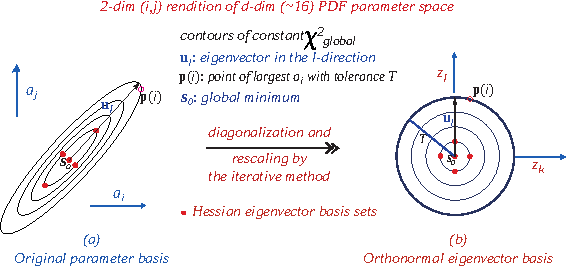
\includegraphics[width=1.0\textwidth]{figures/pdf_constraints/hessianmethod.pdf}
  \caption[Transformation of the parameter basis to the eigenvector basis]
    {Transformation from the original parameter basis to the orthonormal
    eigenvector basis. The uncertainty on the PDFs can be propagated to a
    physical quantity $X$ using these eigenvector PDF sets which are mutually
    uncorrelated. Taken from~\cite{Pumplin:2001ct}.}
    \label{fig:eigenvector_basis_set}
\end{figure}

Using an iterative method, the downwards and upwards variation of each
eigenvector corresponding to $\chisq = \chisq_{\mathrm{min}} + 1$ is calculated.
Since the eigenvectors are orthogonal, the eigenvector variation PDFs correspond
to independent sources of uncertainty on the PDFs. The asymmetric uncertainties
$\Delta X_{\mathrm{exp}}^+$ and $\Delta X_{\mathrm{exp}}^-$ on a quantity of
interest $X$ are evaluated as
%
\begin{align*}
  \Delta X^+_{\mathrm{exp}} &= \sqrt{\sum_i^{N_{\mathrm{EV}}} \left[ \max(X_i^{\mathrm{up}}
    -X_0, X_i^{\mathrm{dn}} - X_0, 0)\right]^2}\\
    \Delta X^-_{\mathrm{exp}} &= \sqrt{\sum_i^{N_{\mathrm{EV}}} \left[
    \min(X_i^{\mathrm{up}} - X_0, X_i^{\mathrm{dn}} - X_0,0)\right]^2}\,,
\end{align*}
%
where $X_0$ describes the central prediction and $X_i^{\mathrm{up}}$ and
$X_i^{\mathrm{dn}}$ denote the result using the upwards and downwards variation of
the eigenvector PDF set $i$ of the $N_{\mathrm{EV}}$ eigenvectors in the PDF
set. $X$ may be a cross section calculation or the PDFs themselves.

\paragraph{Model uncertainties} 
The uncertainties of several input parameters in the PDF fits are combined into
one PDF model uncertainty. For the evaluation of the model uncertainties the
following variations on the input parameters are considered, following the
prescription of the HERAPDF 2.0 publication.:
%
\begin{itemize}
\item The assumption is made that the shape of the strange quark PDF follows the
  shape of the down-like sea quark PDF. Thus, the strange quark PDF is not
  fitted but determined as a fraction of the $x\overline{D}$ PDF. The strangeness fraction
  $f_s$, by default set equal to $0.40$, is varied between $0.30$ and $0.50$.
  \item The b-quark mass is set to $\SI{4.5}{\GeV}$ and varied between
  $\SI{4.25}{\GeV}$ and $\SI{4.75}{\GeV}$.
  \item The c-quark mass, set by default to $\SI{1.47}{\GeV}$ is varied between
  $\SI{1.41}{\GeV}$ and $\SI{1.53}{\GeV}$.
  \item The minimum $Q^2$ value for DIS data used in the fit,
    $Q^2_\mathrm{min}=\SI{7.5}{\GeVsq}$, is varied to $Q^2_\mathrm{min} =
    \SI{5.0}{\GeV\squared}$ and $Q^2_\mathrm{min} = \SI{10.0}{\GeV\squared}$.
\end{itemize}
%
The model uncertainty is evaluated in the same way as the PDF eigenvectors.
The variation of each input parameter is treated as an independent variation
leading to the definition of the asymmetric model uncertainty as:

\begin{align*}
  \Delta X^+_{\mathrm{mod}} &= \sqrt{\sum_i^{N_{\mathrm{par}}} \left[ \max(X_i^{\mathrm{up}}
    -X_0, X_i^{\mathrm{dn}} - X_0, 0)\right]^2}\\
    \Delta X^-_{\mathrm{mod}} &= \sqrt{\sum_i^{N_{\mathrm{par}}} \left[ \min(X_i^{\mathrm{up}} - X_0, X_i^{\mathrm{dn}} - X_0,0)\right]^2}
\end{align*}

\paragraph{Parametrization uncertainty}

To estimate the influence of the initial PDF parametrization on the fit result, a
more flexible function form is used. Using the general
parametrizations for the gluon PDF $xg(x)$
%
\begin{align*}
   xg(x) &= A_g x^{B_g} (1-x)^{C_g} (1  + D_g x + E_g x^2) - A'_g x^{B'_g} (1-x)^{C'_g}\\
\intertext{and the quark PDFs $xf(x)$}
   xf(x) &= A_{f}  x^{B_{f}} (1-x)^{C_{f}} (1 + D_{f}x + E_{f}x^2),
\end{align*}
%
it is studied if the inclusion of additional parameters in the fit yields
a different result. Each parameter is successively added in the PDF fit and the
envelope of all changes to the PDF shape are combined into one parametrization
uncertainty. Furthermore, the variation of the starting scale $Q_0^2$ to
\SI{1.6}{\GeV\squared} and \SI{2.2}{\GeV\squared} is treated as an 
parametrization variation.

\begin{align*}
  \Delta X^+_{\mathrm{par}} &= \max_{i}^{n} \left[ X^i - X^0, 0 \right]\\
  \Delta X^-_{\mathrm{par}} &= \max_{i}^{n} \left[ X^0 - X^i, 0 \right]
\end{align*}


\subsection{Definition of the Goodness-of-Fit Estimator}
\label{sec:chi2_definition}

The minimization procedure of the PDF fit is using a least-squares method. The \chisq is
calculated with the data points $D_i$ and the theoretical prediction $T_i$. The
$K$  correlated systematic uncertainties $\beta_{k}$ are treated using nuisance parameters
$_k$ in the fit, which are applied to the theoretical prediction, in order to avoid the bias from
multiplicative data uncertainties, see~\cite{Lyons:1989gh}. The \chisq is
defined as
%
\begin{align*}
  \chi^2 = &\sum_{ij}^N \left(D_i - T_i - \sum_k^K r_k \beta_{ik}\right) \mathrm{C}_{ij}^{-1}
  \left(D_j - T_j - \sum_k^K r_k \beta_{jk} \right) + \sum_k^K r_k^2\\
  &+ \sum_j \ln \frac{\Delta_{i,\mathrm{stat}}^2 D_j T_j + \Delta_{i,\mathrm{uncor}}^2 T_i^2}{\left( \Delta_{i,\mathrm{stat}}^2 + \Delta_{i,\mathrm{uncor}}^2 \right) D_i^2}
  \label{chi2_nuisance}
\end{align*}
%
where $C_{ij}^{-1}$ is the inverse covariance matrix of the uncorrelated or
partly correlated systematic and statistical uncertainties and $\Delta_\mathrm{stat}$ and
$\Delta_\mathrm{uncor}$ are the diagonal elements of the statistical and
uncorrelated uncertainty. All fully correlated uncertainties are treated using
nuisance parameters. The log term in the \chisq definition is an additional
correction term which accounts for a bias that arises from the treatmen of
poisson-like uncertainties in a \chisq fit expecting Gaussian distributed
uncertainties.

More information can be found
in~\cite{Alekhin:2014irh,Abramowicz:2015mha}. An advantage of such a \chisq
definition with nuisance parameters is the possibility to study the pulls of
each systematic source after the fit.

\subsection{Treatment of Systematic Uncertainties}
\label{section:cmsdatauncertainties}

Since the correlated sources of uncertainty are treated using nuisance
parameters in the \chisq formula, the pull of each source can be examined.
Tab.~\ref{tab:pdfconstraints:nuisance} shows the 27 sources of systematic
uncertainty and their pulls. Most of the systematic sources shift by less than
one standard deviation. Three sources exhibit larger shifts. While this not
surprising due to the Gaussian distribution of the pulls, no unambiguous
reason for their behavior could be identified. However, the size of these
uncertainty sources is rather small compared to the dominant sources of
uncertainty so that no significant influence on the fit is expected.

\todo{update in the end again with final values}
\begin{table}[htbp]
  \caption[Nuisance parameters obtained after the PDF fit]{Nuisance parameters
  obtained after the PDF fit. The shift of each nuisance parameter is reported
in standard deviations of its represented uncertainty source. Most of the pulls cause shifts by less than a standard deviation.}
  \label{tab:pdfconstraints:nuisance}
  \centering
  \begin{tabular}{lrlr}
    \toprule
    \textbf{Systematic source} & \textbf{Shift in $\sigma$} & \textbf{Systematic source} & \textbf{Shift in $\sigma$}\rbthm\\\midrule
    \textsc{AbsoluteScale}     &  -0.33                    & \textsc{RelativeFSR}       &   0.97        \rbtrr\\
    \textsc{AbsoluteStat}      &  -0.29                    & \textsc{RelativeStatEC2}   &   0.52         \rbtrr\\
    \textsc{AbsoluteMPFBias}   &  -0.57                    & \textsc{RelativeStatHF}    &   0.08        \rbtrr\\
    \textsc{Fragmentation}     &  -0.22                    & \textsc{RelativeStatFSR}   &   -0.23        \rbtrr\\
    \textsc{SinglePionECAL}    &  -0.20                    & \textsc{PileUpDataMC}      &   0.03         \rbtrr\\
    \textsc{SinglePionHCAL}    &  -0.75                    & \textsc{PileUpPtRef}       &   -0.27        \rbtrr\\
    \textsc{FlavorQCD}         &  -0.77                    & \textsc{PileUpPtBB}        &   -2.57       \rbtrr\\
    \textsc{RelativeJEREC1}    &  0.12                     & \textsc{PileUpPtEC1}       &   1.11         \rbtrr\\
    \textsc{RelativeJEREC2}    &  0.04                     & \textsc{PileUpPtEC2}       &   0.37        \rbtrr\\
    \textsc{RelativeJERHF}     &  0.14                     & \textsc{PileUpPtHF}        &   0.00        \rbtrr\\
    \textsc{RelativePtBB}      &  -0.74                    & \textsc{NPErr}             &   1.04         \rbtrr\\
    \textsc{RelativePtEC1}     &  0.54                     & \textsc{JERerr}            &   0.62        \rbtrr\\
    \textsc{RelativePtEC2}     &  -0.72                    & \textsc{Lumi}              &   0.84        \rbtrr\\
    \textsc{RelativePtHF}      &  0.00                     &                            &           \rbtrr\\
    \bottomrule
  \end{tabular}
\end{table}

\section{Constraints on PDFs of the Triple-Differential Dijet Cross Section}
\label{section:cmsjets2011_pdfconstraints}

The quality of the fit with and without including the dijet measurement is
reported in Table~\ref{tab:fit:results}. The partial \chisq per data point for
each data set as well the \chisq per \ndof for all data sets demonstrate
the compatibility of the CMS dijet measurement and the DIS data from the HERA
experiments. 

\todo{update in the end again with final values}
\begin{table}[htbp]
\small
\setlength\tabcolsep{2.5pt} 
  \caption[Fit quality in the HERA DIS and combined fit]{The Partial \chisq's  for each data set in the HERA DIS (middle
    section) or the combined fit including the triple-differential dijet data
    (right section) are shown.
    \ndata is the number of data points available for the determination of
    the 13 parameters. The bottom two lines show the total \chisq and
    \chisqndof. The difference between the sum of all
    \chipsq and the total \chisq for the combined fit is attributed to
    the nuisance parameters.}
  \label{tab:fit:results}
  \centering
  \begin{tabular}{lrrcrc}
    \toprule
    \multicolumn{2}{c}{} &
    \multicolumn{2}{c}{\textbf{HERA data}} &
    \multicolumn{2}{c}{\textbf{HERA \& CMS data}}\rbtrr\\\cmidrule(l){3-6}
    \textbf{data set} &
    \multicolumn{1}{c}{\ndata} &
    \multicolumn{1}{c}{\chipsq} &
    \multicolumn{1}{c}{\chipsqndata} &
    \multicolumn{1}{c}{\chipsq} &
    \multicolumn{1}{c}{\chipsqndata}\rbthm\\\midrule
    CC HERA-I+II e-p.                                   & 42  & 54.64  & 1.30 & 51.88  & 1.24 \rbtrr\\
    CC HERA-I+II e+p.                                   & 39  & 37.47  & 0.96 & 37.47  & 0.96 \rbtrr\\
    NC HERA-I+II e-p.                                   & 159 & 216.72 & 1.36 & 219.66 & 1.38 \rbtrr\\
    NC HERA-I+II e+p. $E_{\mathrm{p}} = \SI{460}{\GeV}$ & 187 & 204.97 & 1.10 & 205.65 & 1.10 \rbtrr\\
    NC HERA-I+II e+p. $E_{\mathrm{p}} = \SI{575}{\GeV}$ & 234 & 196.90 & 0.84 & 198.39 & 0.85 \rbtrr\\
    NC HERA-I+II e+p. $E_{\mathrm{p}} = \SI{820}{\GeV}$ & 63  & 61.68  & 0.98 & 61.83  & 0.98 \rbtrr\\
    NC HERA-I+II e+p. $E_{\mathrm{p}} = \SI{920}{\GeV}$ & 332 & 376.03 & 1.13 & 401.72 & 1.21 \rbtrr\\
    CMS Triple-Differential Dijets                      & 111 & ---    & ---  & 99.10  & 0.89
    \rbtrr\\\bottomrule
    \textbf{data set(s)} & \ndof &
    \multicolumn{1}{c}{\chisq} &
    \multicolumn{1}{c}{\chisqndof} &
    \multicolumn{1}{c}{\chisq} &
    \multicolumn{1}{c}{\chisqndof}\rbthm\\\midrule
    HERA data                       & 1043 & 1208.10 & 1.16  &  --- &  --- \rbtrr\\
    HERA \& CMS data                & 1154 &    --- &  --- & 1341.54 & 1.16 \rbtrr\\
    \bottomrule
  \end{tabular}
\end{table}


The resulting PDFs for the gluon, u valence, d valence and sea quark for a fit
with and without the CMS dijet data are shown next to each other in the
Figs.~\ref{fig:pdfconstraints:split:gluonqsea:19}--\ref{fig:pdfconstraints:split:dvaluval:19}
with a breakdown of the three sources of uncertainty. A direct comparison of
the PDFs with total uncertainties can be found in the appendix in the
Figs.~\ref{fig:pdfconstraints:direct:19}--\ref{fig:pdfconstraints:direct:10000}.
The uncertainty breakdown in Fig.~\ref{fig:pdfconstraints:split:gluonqsea:19} reveals the large impact of
the dijet data. The uncertainty of the gluon PDF is reduced over almost the
whole range in $x$. In the high-$x$ region, the experimental uncertainty is
reduced, while most changes in the low-$x$ region can be attributed to the model
uncertainties. The large changes of uncertainties come
along with a noticeably change of the high-$x$ gluon PDF shape. The gluon PDF is
harder compared to the fit with HERA DIS data alone. Similar changes were
observed before, \eg in~\cite{Khachatryan:2014waa}.

The changes of the sea quark PDF, defined as $x\Sigma=2(x\overline U + x
\overline D + x\overline s)$, are much less pronounced.
The experimental and model uncertainties are reduced in the high-$x$ region.
The u valence and d valence quark PDFs also show uncertainty reductions over
a large $x$-range, most pronounced at high $x$. The uncertainty decrease of the experimental uncertainty is
sizable for high-$x$, while the main differences result from the parametrization
uncertainty, which is significant for the fit with HERA DIS data alone, but
almost completely vanishes in the fit including the CMS dijet data.

In contrast to the previous figures, Fig.~\ref{fig:pdfconstraints:direct:10000}
shows the PDFs after the evolution to the scale $Q^2 = \SI{10000}{\GeV \square}$
which is close to the scale of the measurement. The PDFs exhibit the same
features compared to the starting scale $Q_0$, but even more pronounced.
Finally, an overview of the gluon, sea, u valence and d valence quark PDFs is
given in Fig.~\ref{fig:pdfconstraints:overview:19}. 

The large impact of the data on the PDFs is partly caused by the limited
precision of the fit using HERA DIS data alone. In a global PDF fit, constraints
from other measurements already improve the PDFs, so that not such a strong
impact is expected. However, it was shown in Sec.~\ref{sec:nlo_comparisons} that
the data are sufficiently precise to discriminate between the predictions using
different global PDF sets. Thus, also significant improvements of the global
PDF sets are expected.

\begin{figure}[tbp]
  \centering
  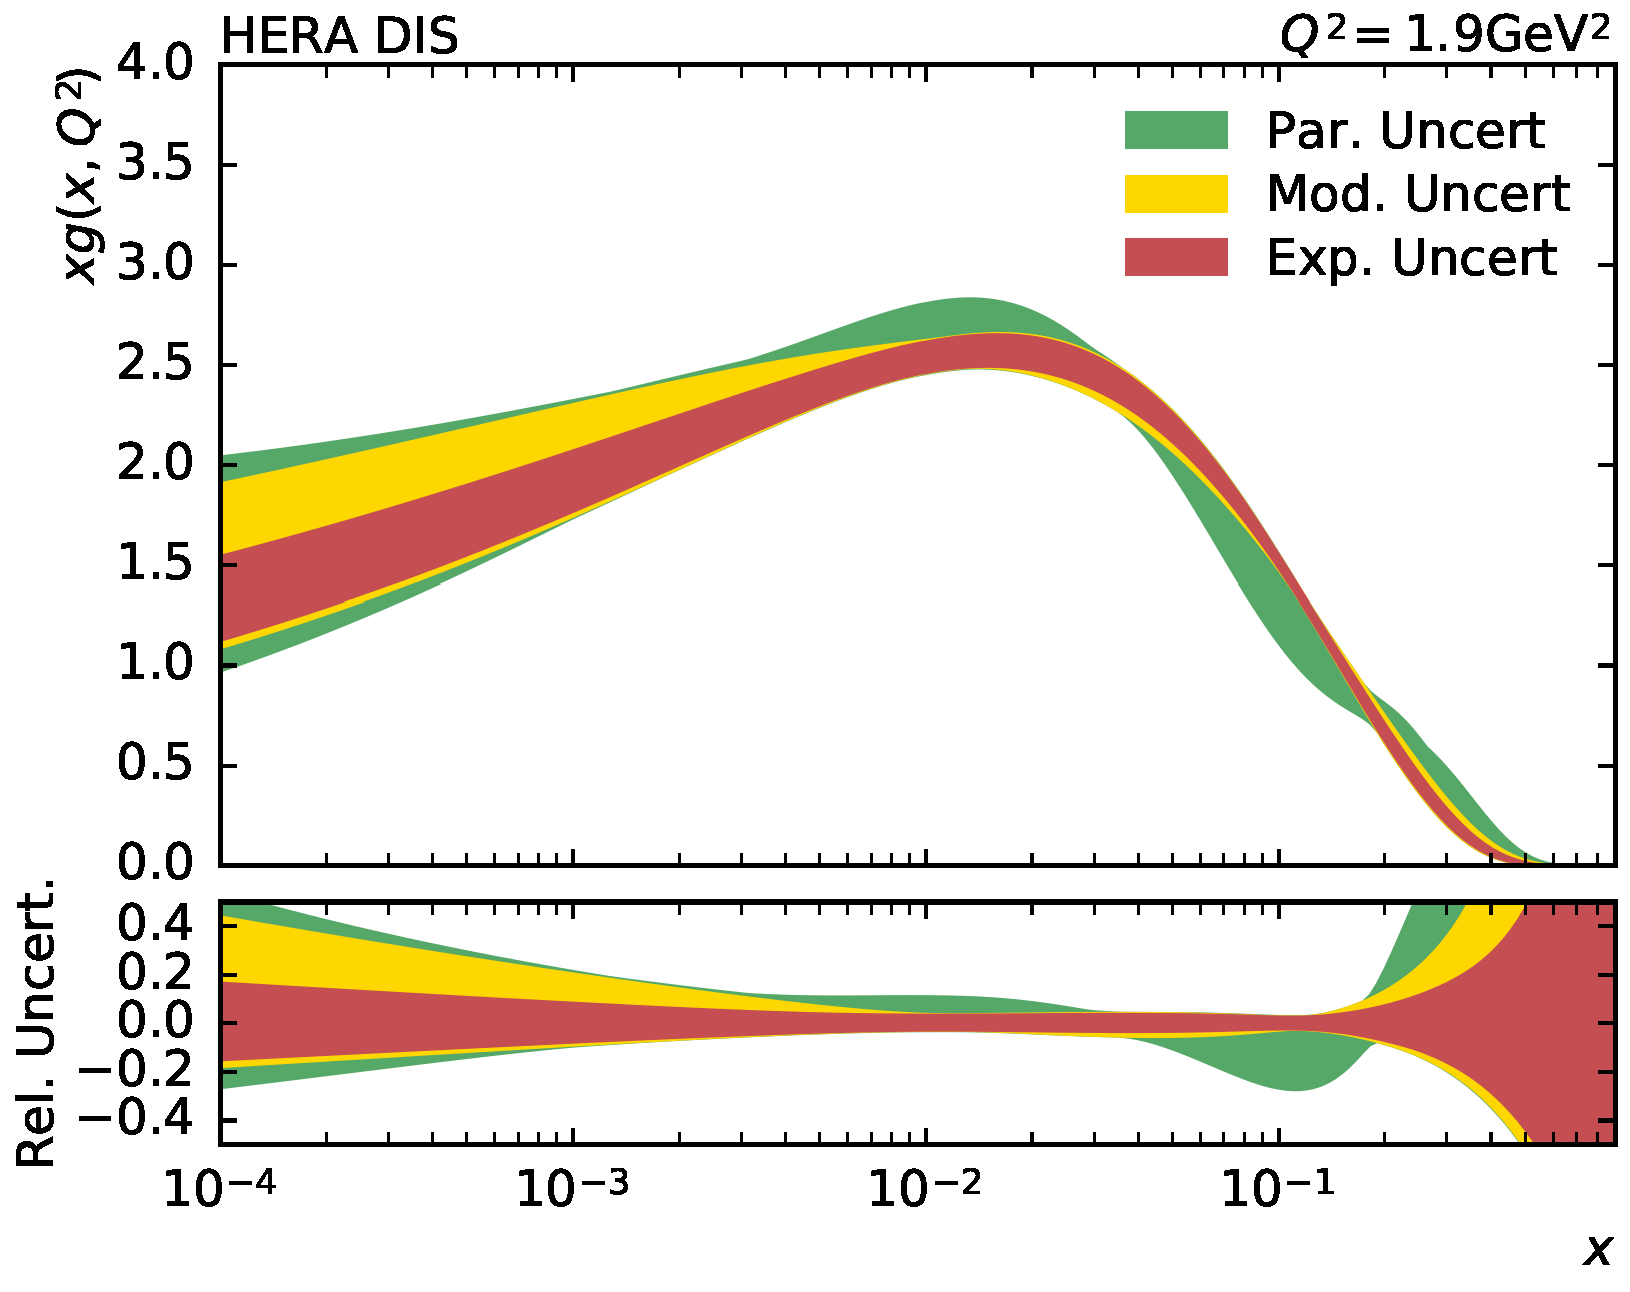
\includegraphics[width=0.48\textwidth]{figures/pdf_constraints/pdfcomp_HFTD_HERA_0_1.9.pdf}\hfill%
  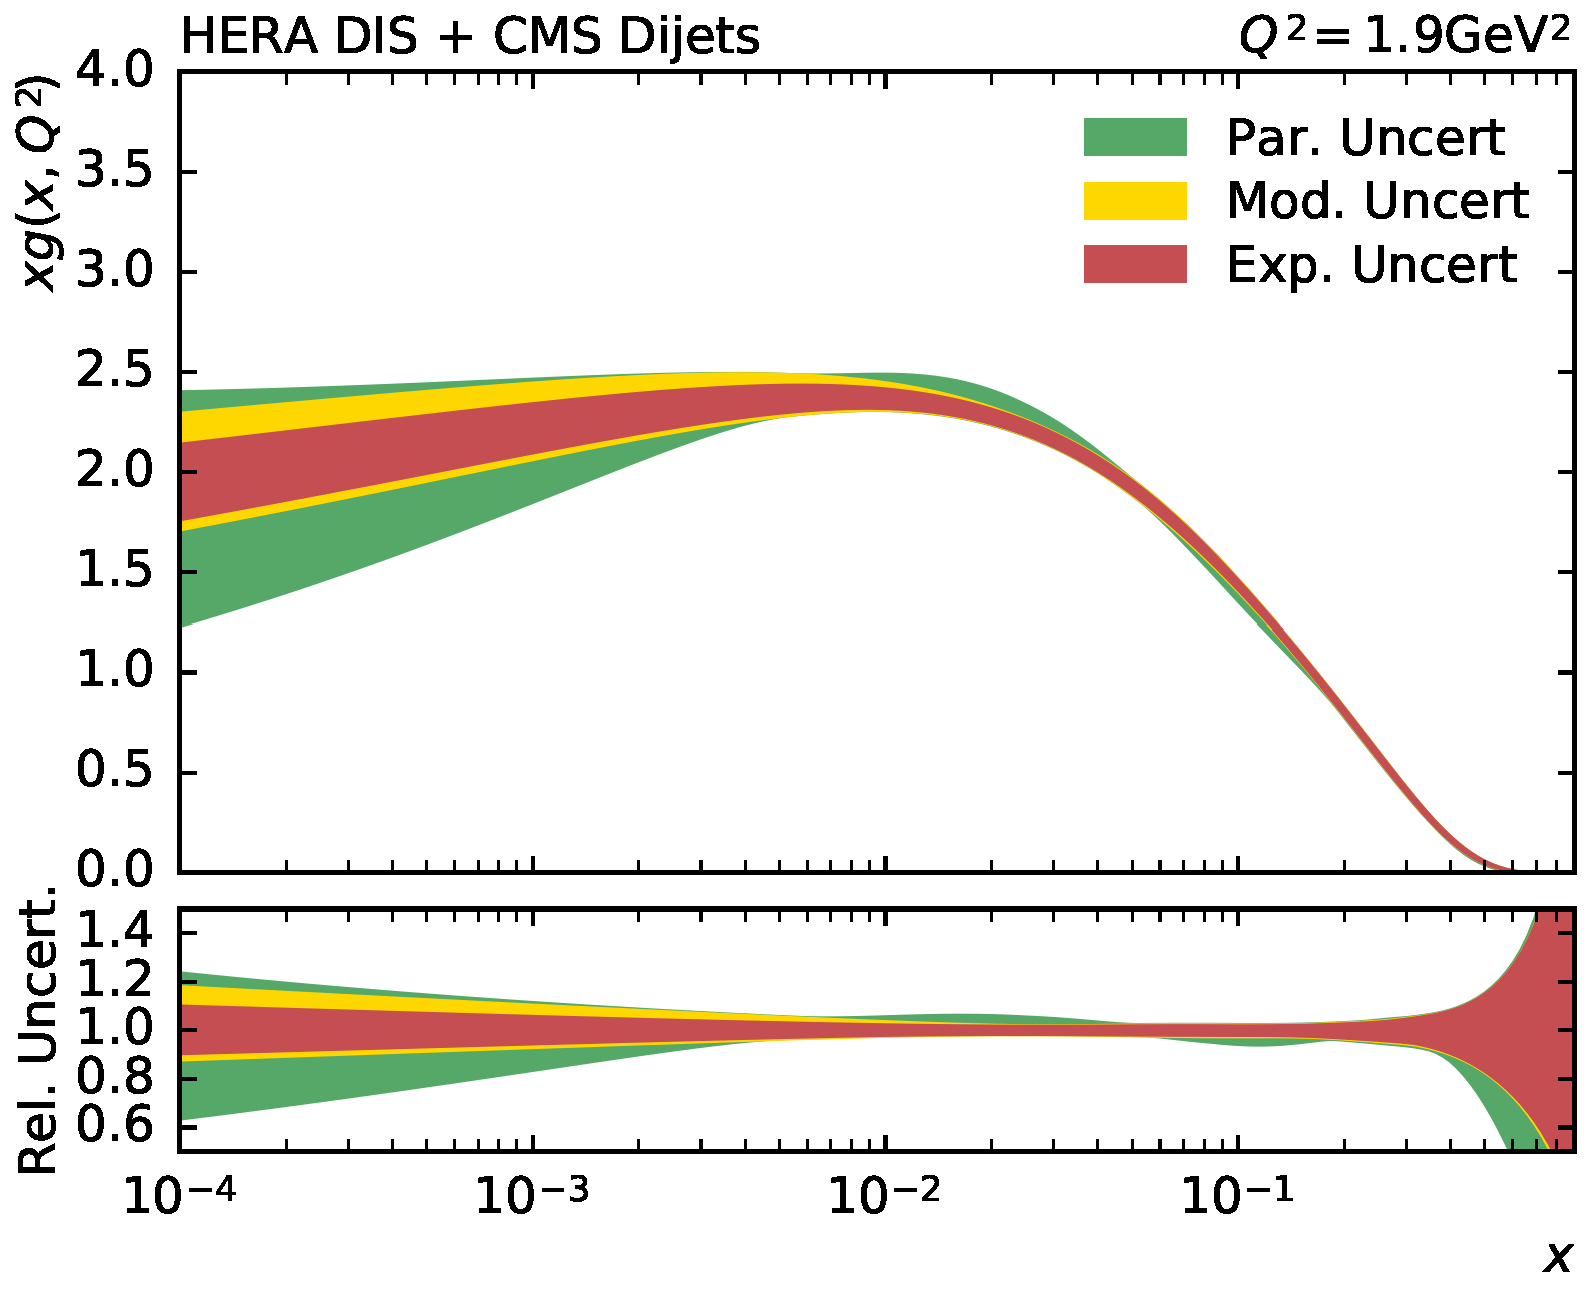
\includegraphics[width=0.48\textwidth]{figures/pdf_constraints/pdfcomp_HFTD_HERACMSTDJETS_0_1.9.pdf}
  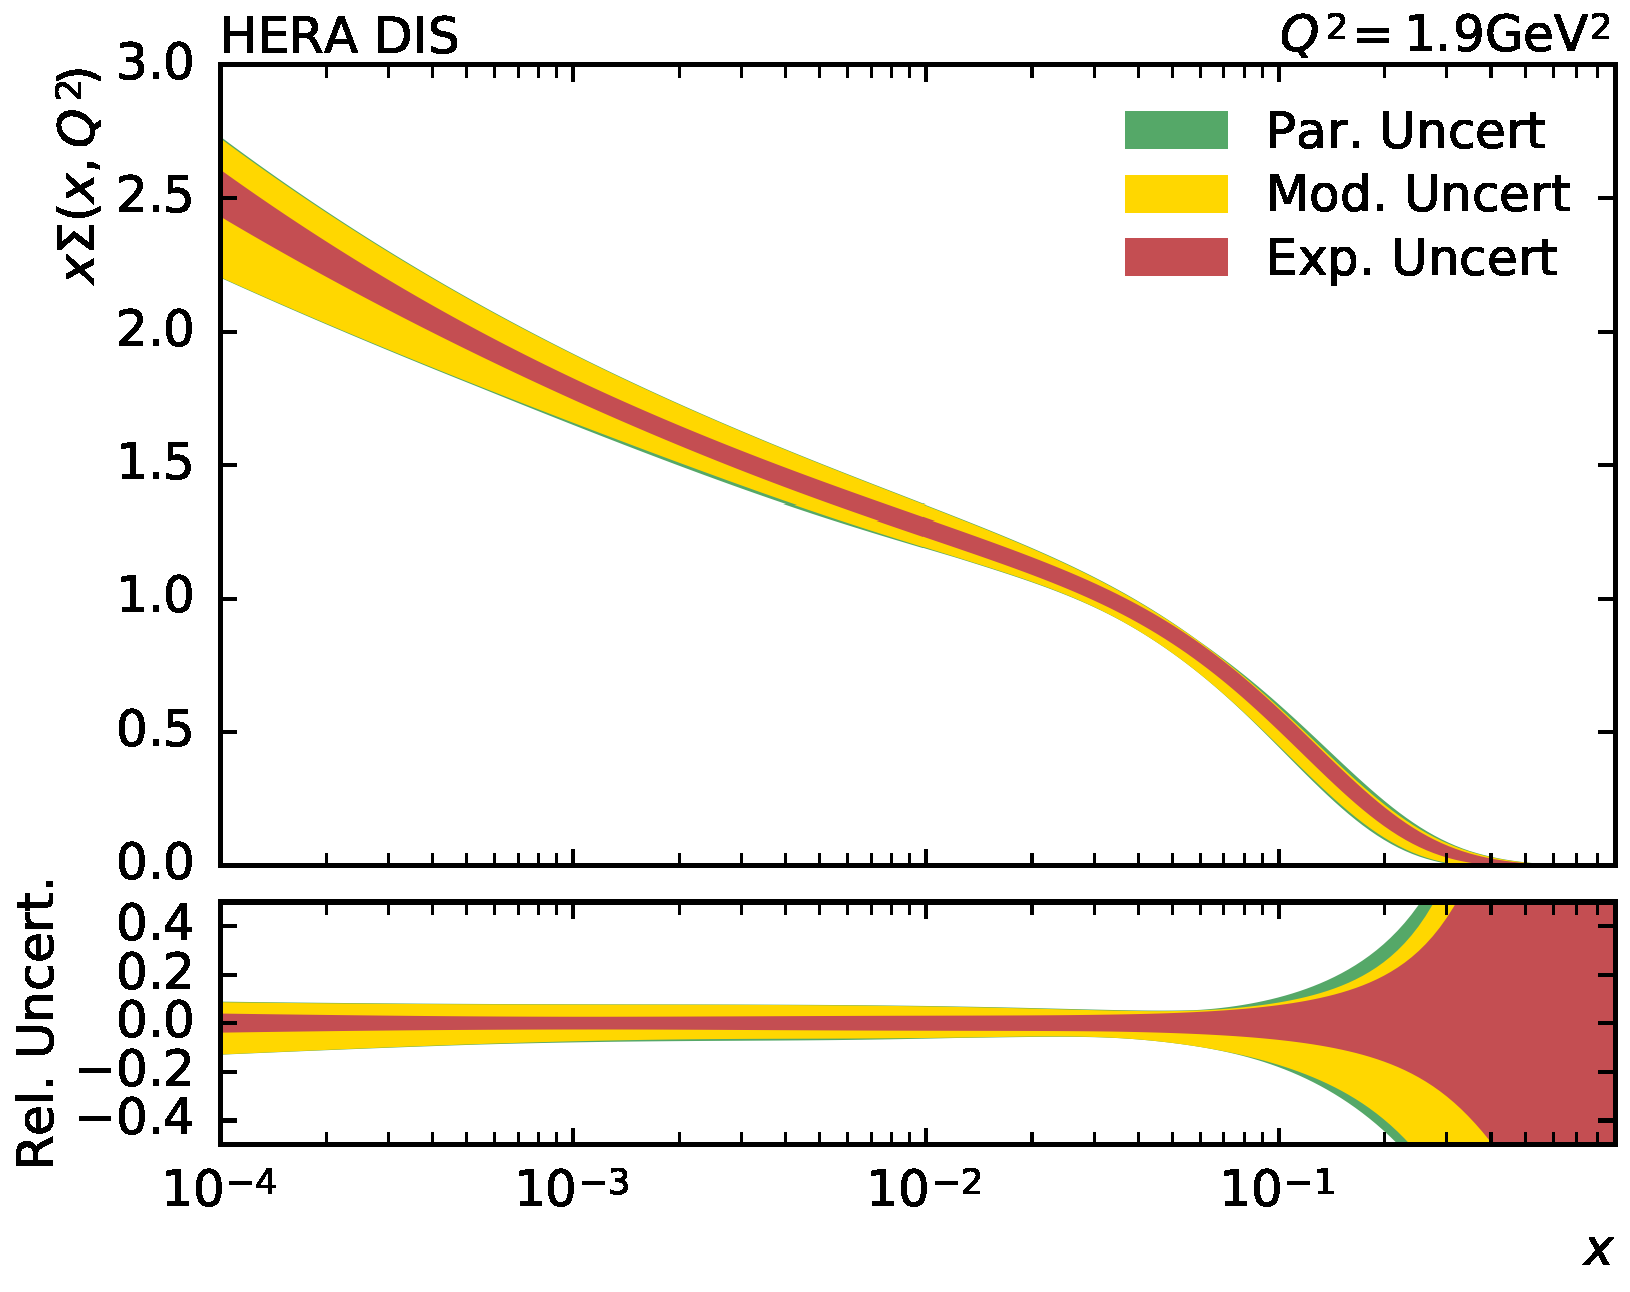
\includegraphics[width=0.48\textwidth]{figures/pdf_constraints/pdfcomp_HFTD_HERA_9_1.9.pdf}\hfill%
  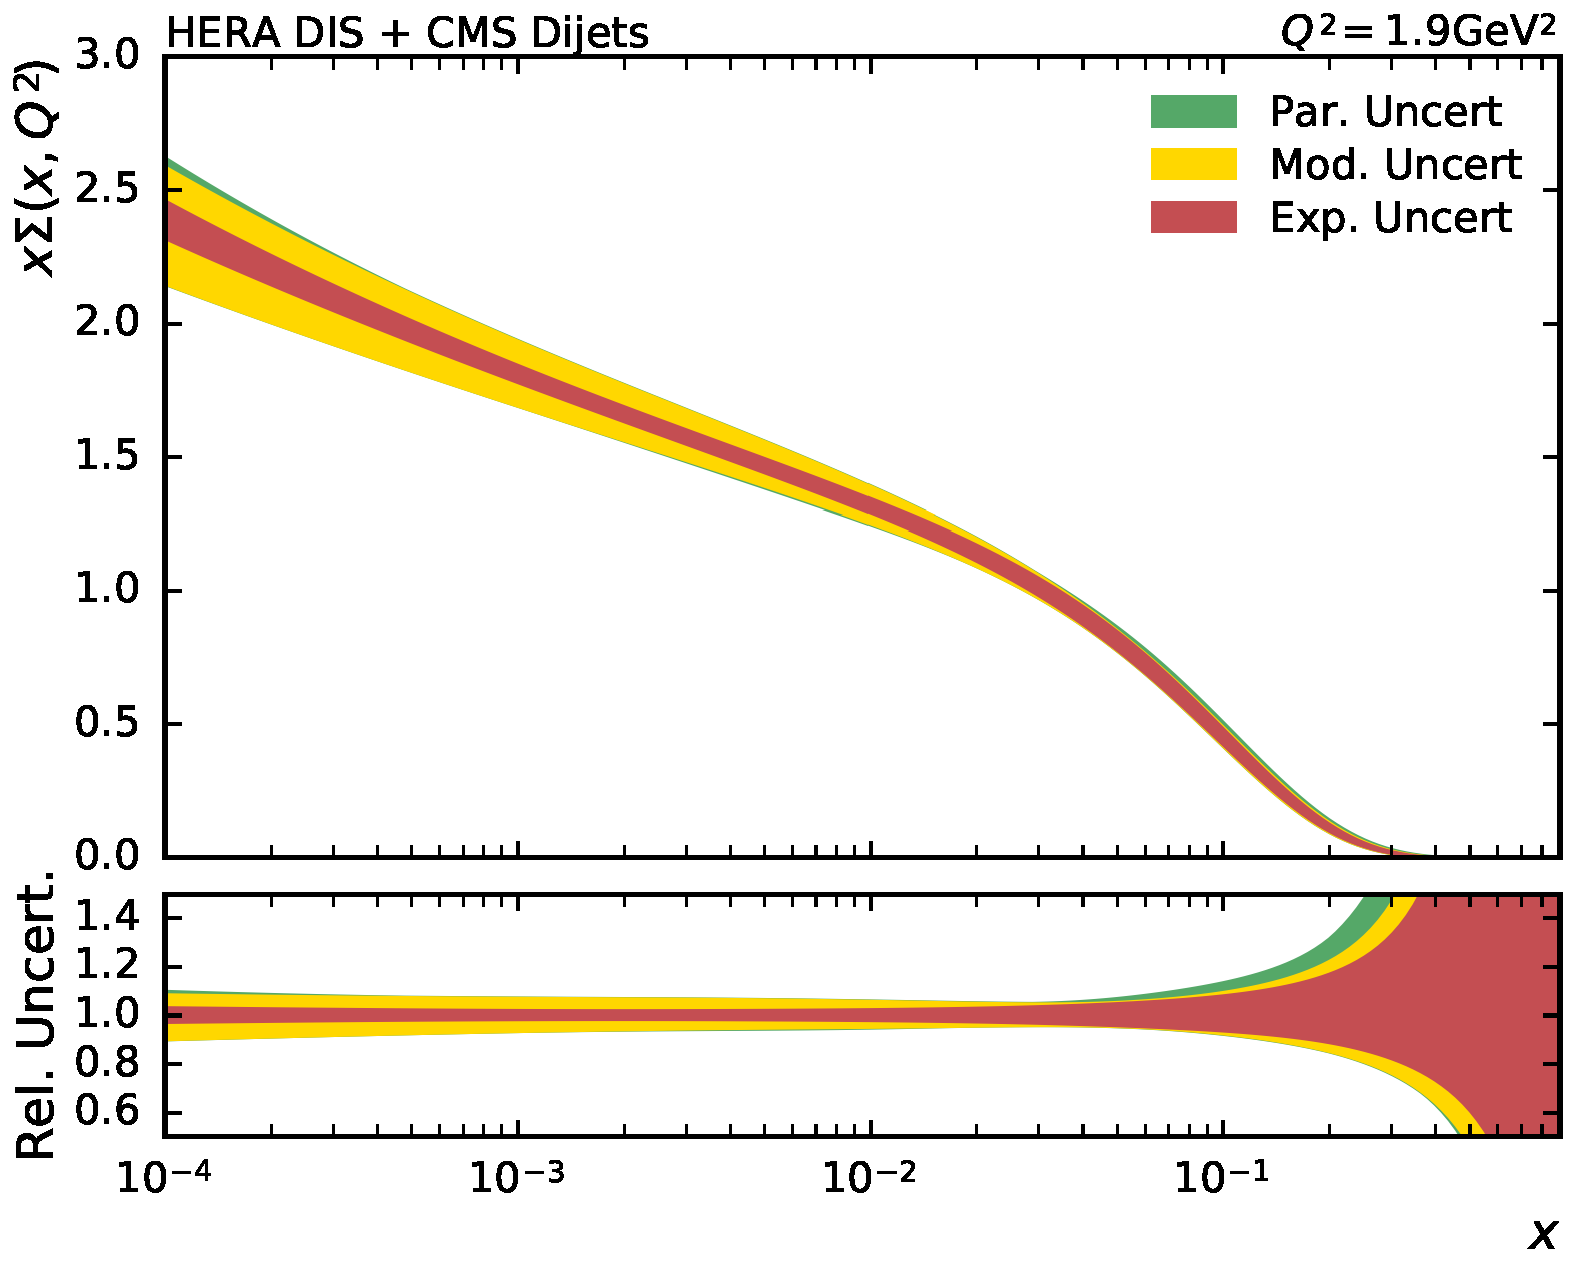
\includegraphics[width=0.48\textwidth]{figures/pdf_constraints/pdfcomp_HFTD_HERACMSTDJETS_9_1.9.pdf}
  \caption[The gluon and sea quark PDFs]{The gluon (top) and sea quark (bottom) PDFs as a function of $x$ as
  derived from HERA inclusive DIS data alone (left) and in combination with
  the CMS dijet data (right). The PDFs are shown at the starting scale $Q^2 =
  \SI{1.9}{\GeV \squared}$. The experimental (inner band), model (middle band)
  and parametrization uncertainties (outer band) are added quadratically to give
  the total uncertainty.}
  \label{fig:pdfconstraints:split:gluonqsea:19}
\end{figure}

\begin{figure}[tbp]
  \centering
  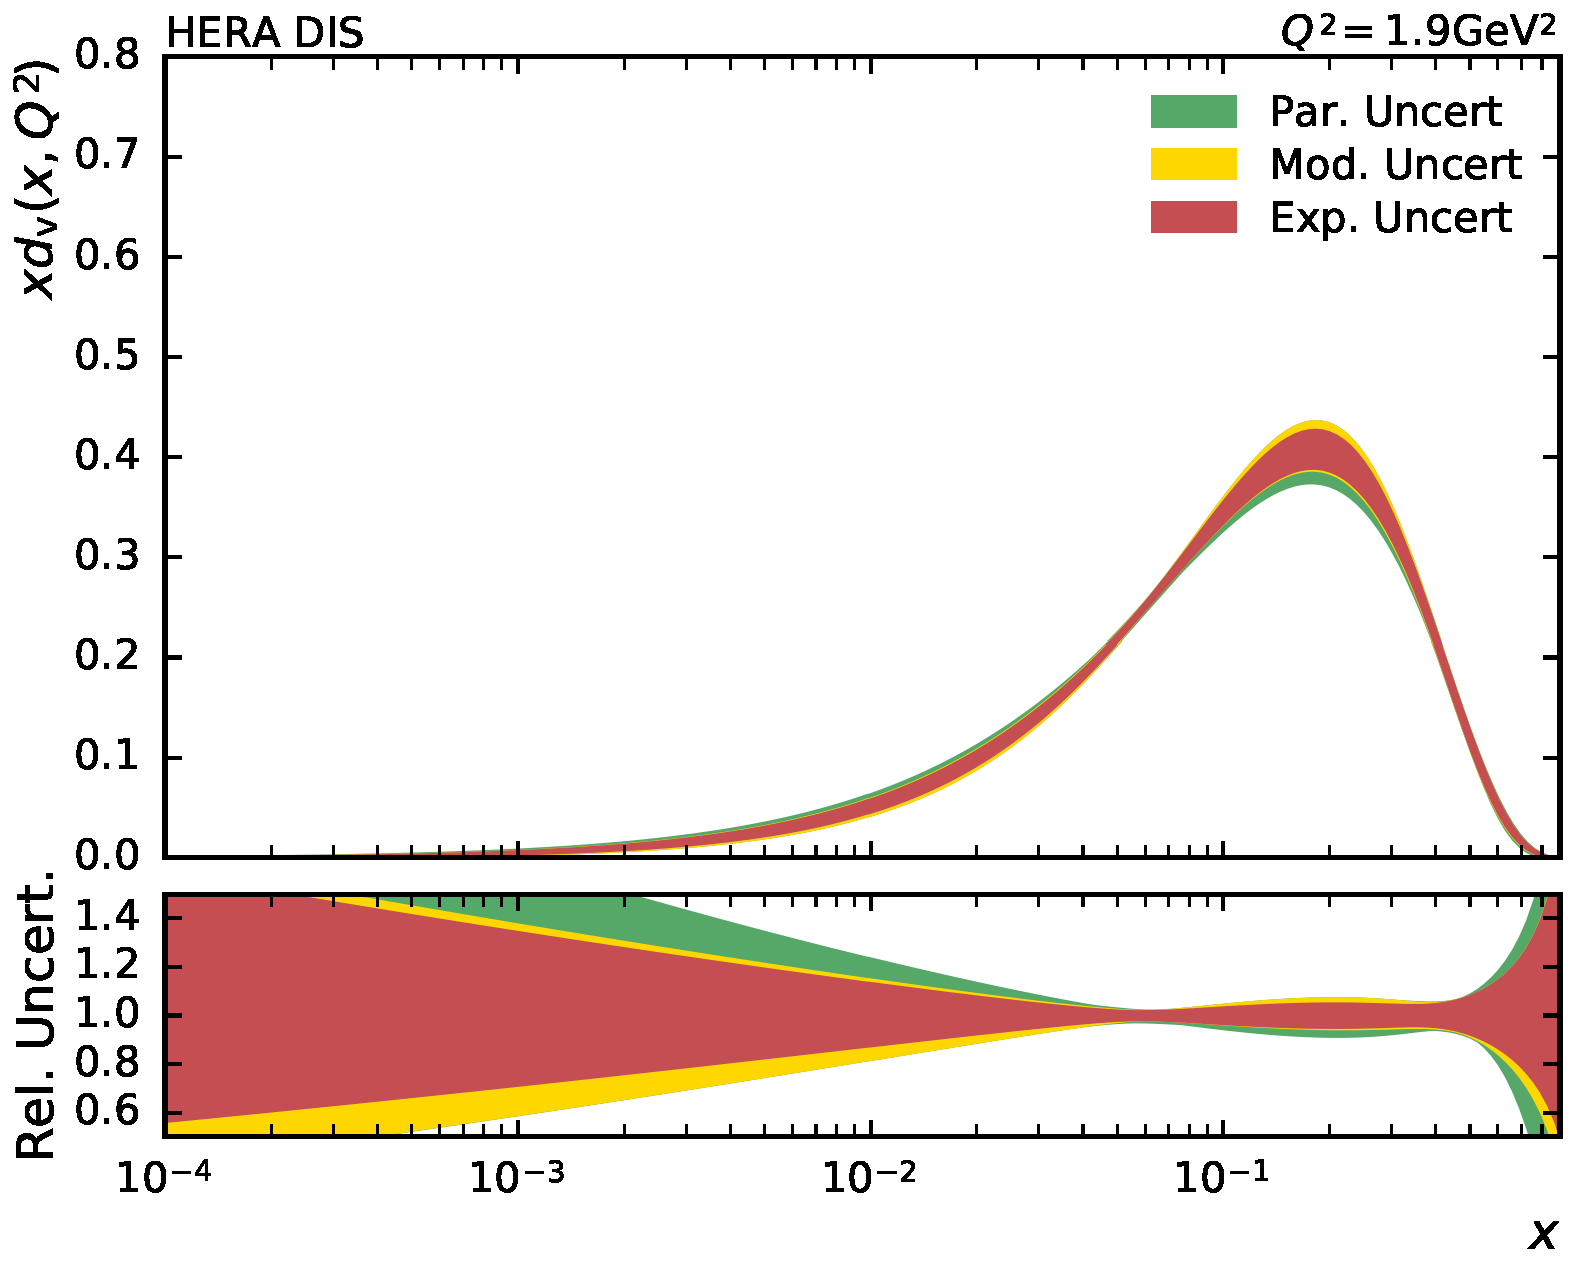
\includegraphics[width=0.48\textwidth]{figures/pdf_constraints/pdfcomp_HFTD_HERA_7_1.9.pdf}\hfill%
  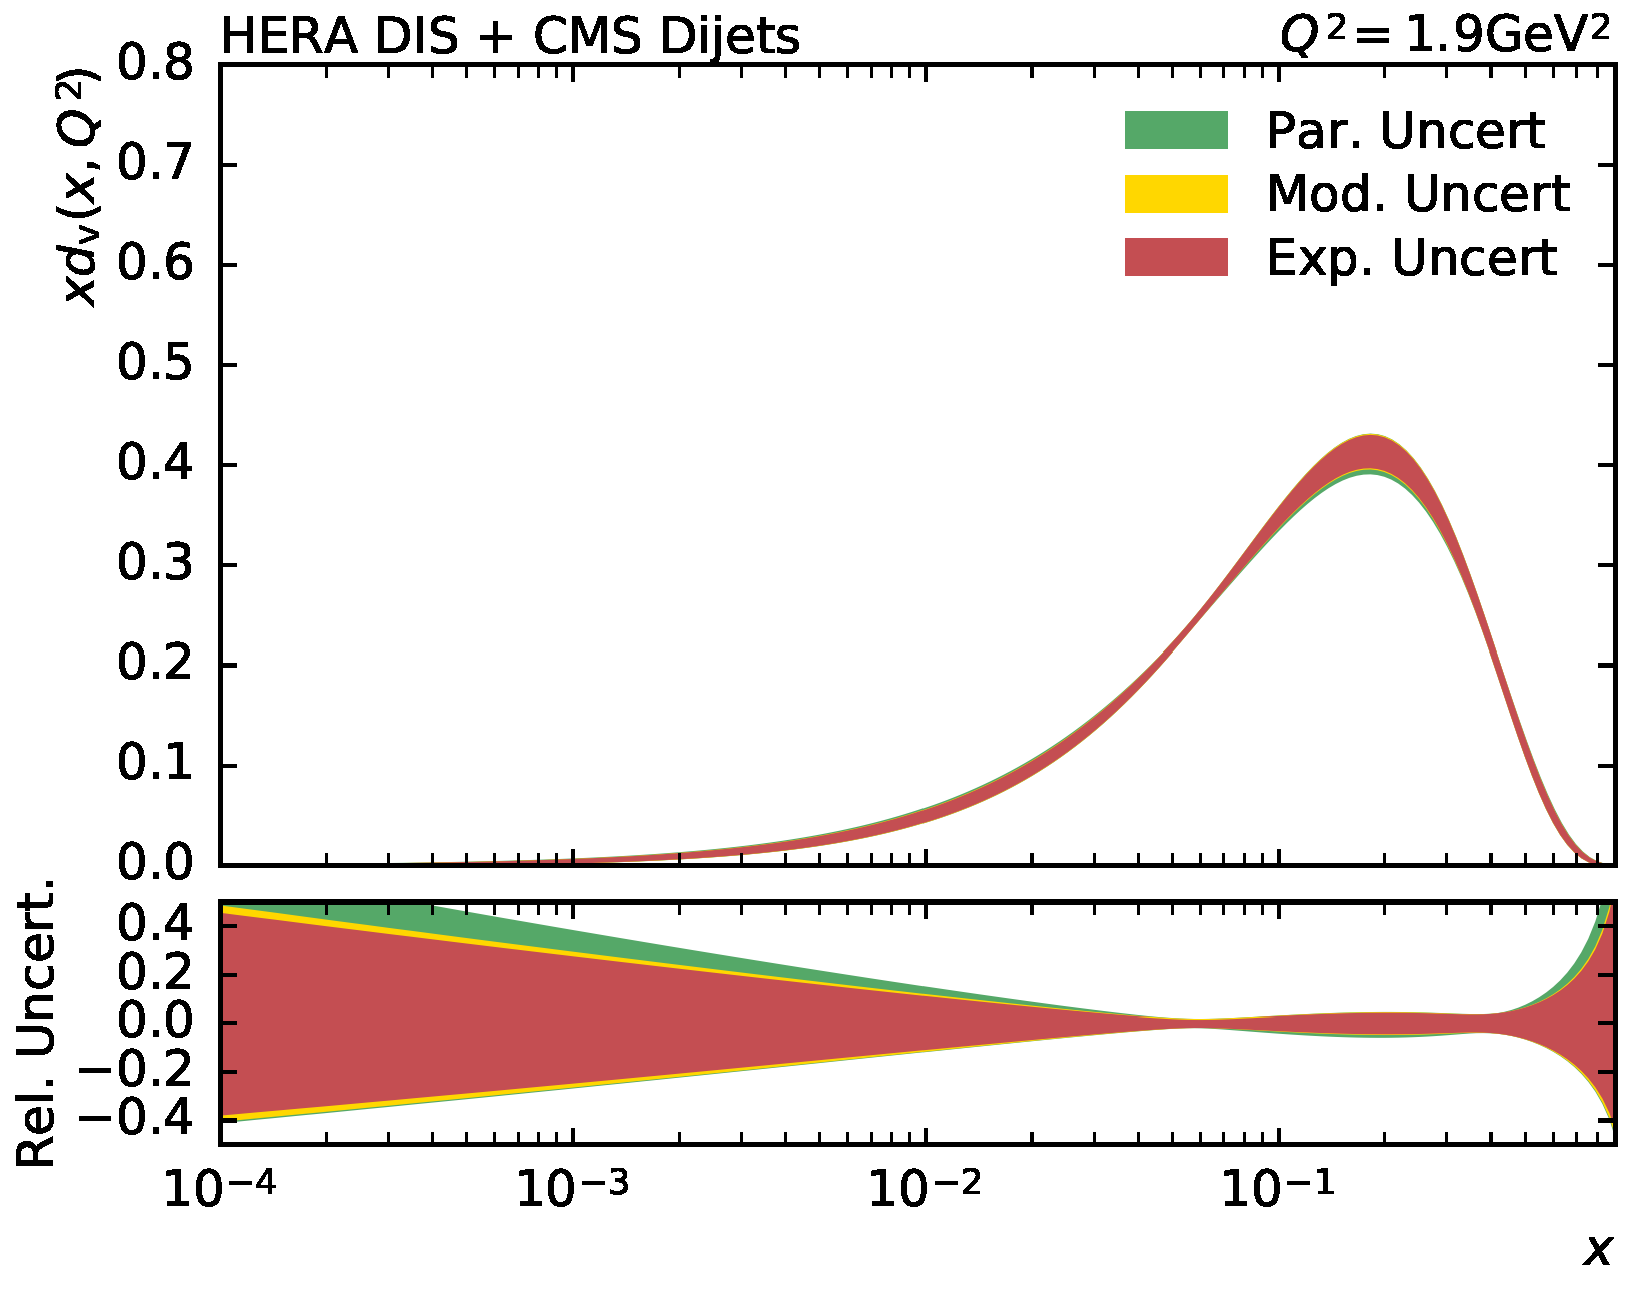
\includegraphics[width=0.48\textwidth]{figures/pdf_constraints/pdfcomp_HFTD_HERACMSTDJETS_7_1.9.pdf}
  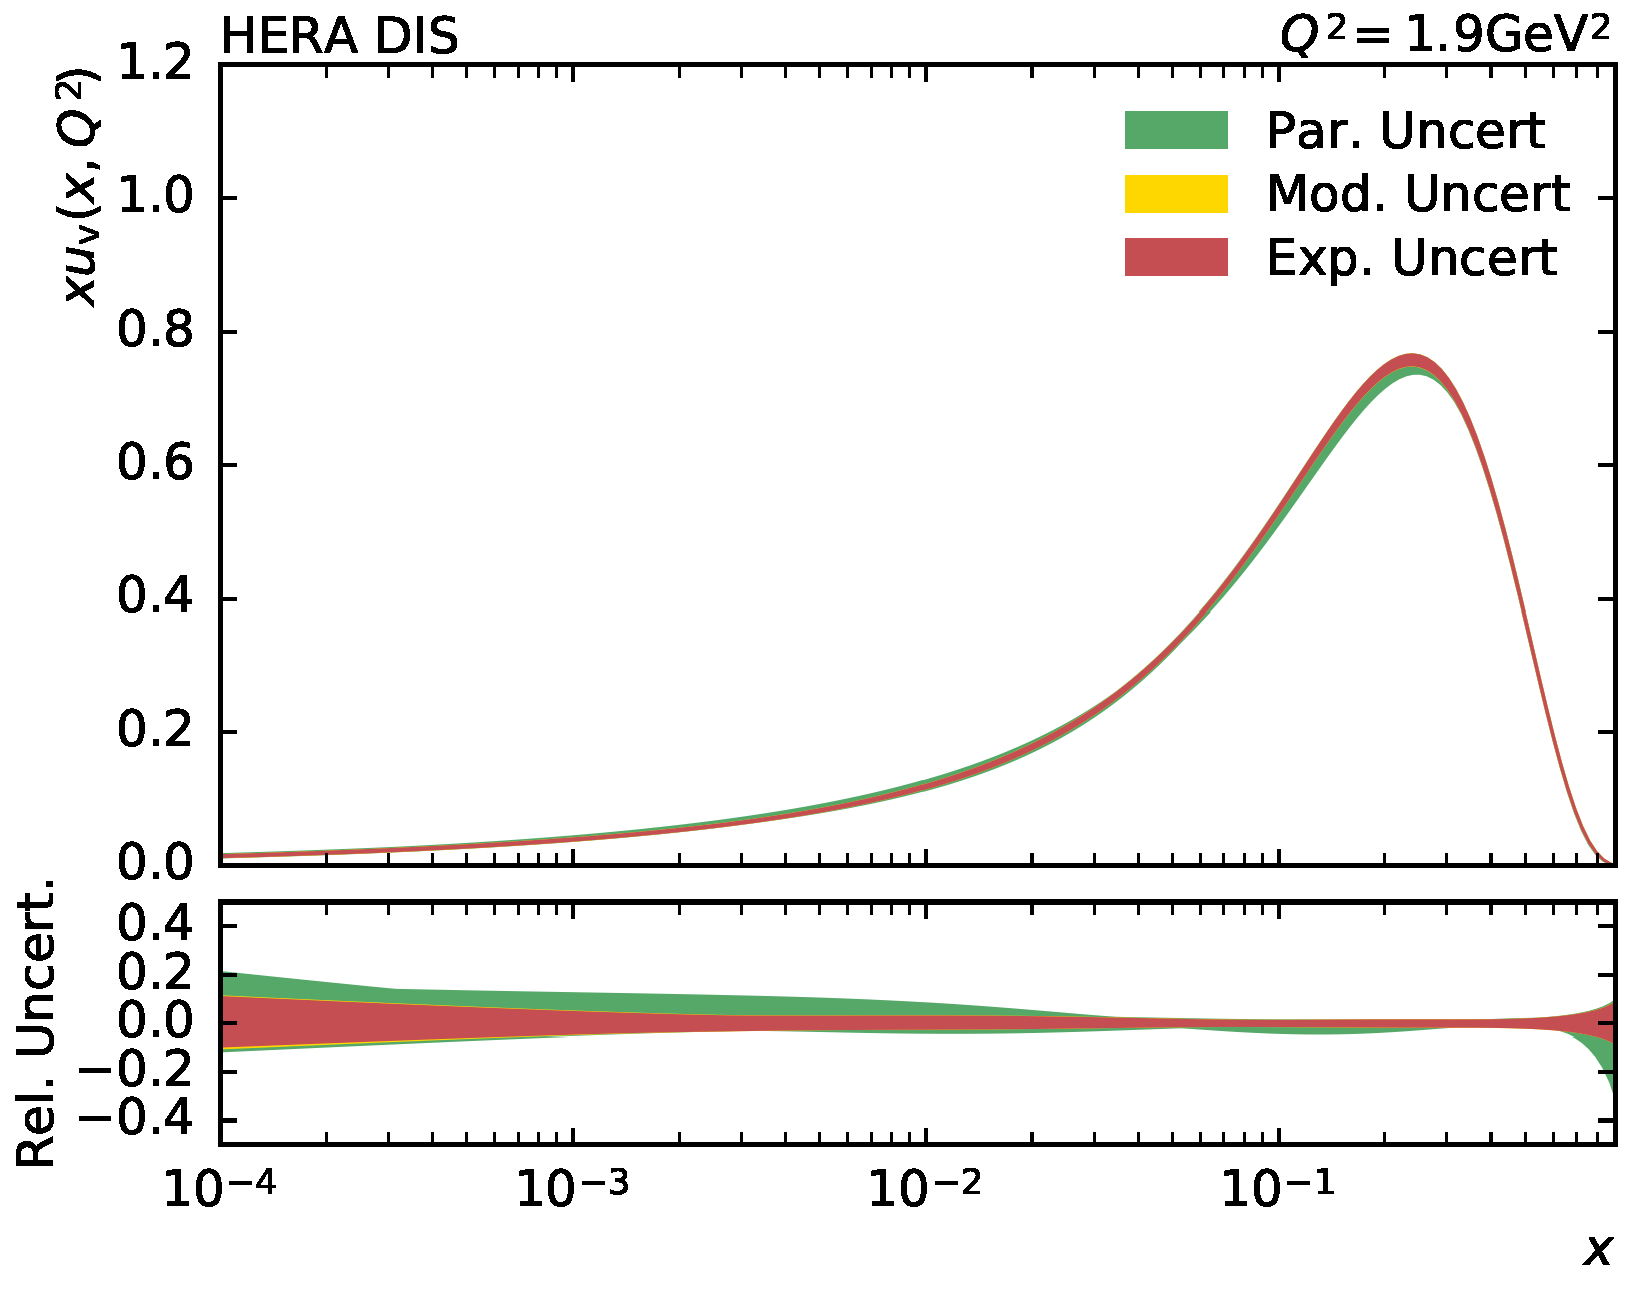
\includegraphics[width=0.48\textwidth]{figures/pdf_constraints/pdfcomp_HFTD_HERA_8_1.9.pdf}\hfill%
  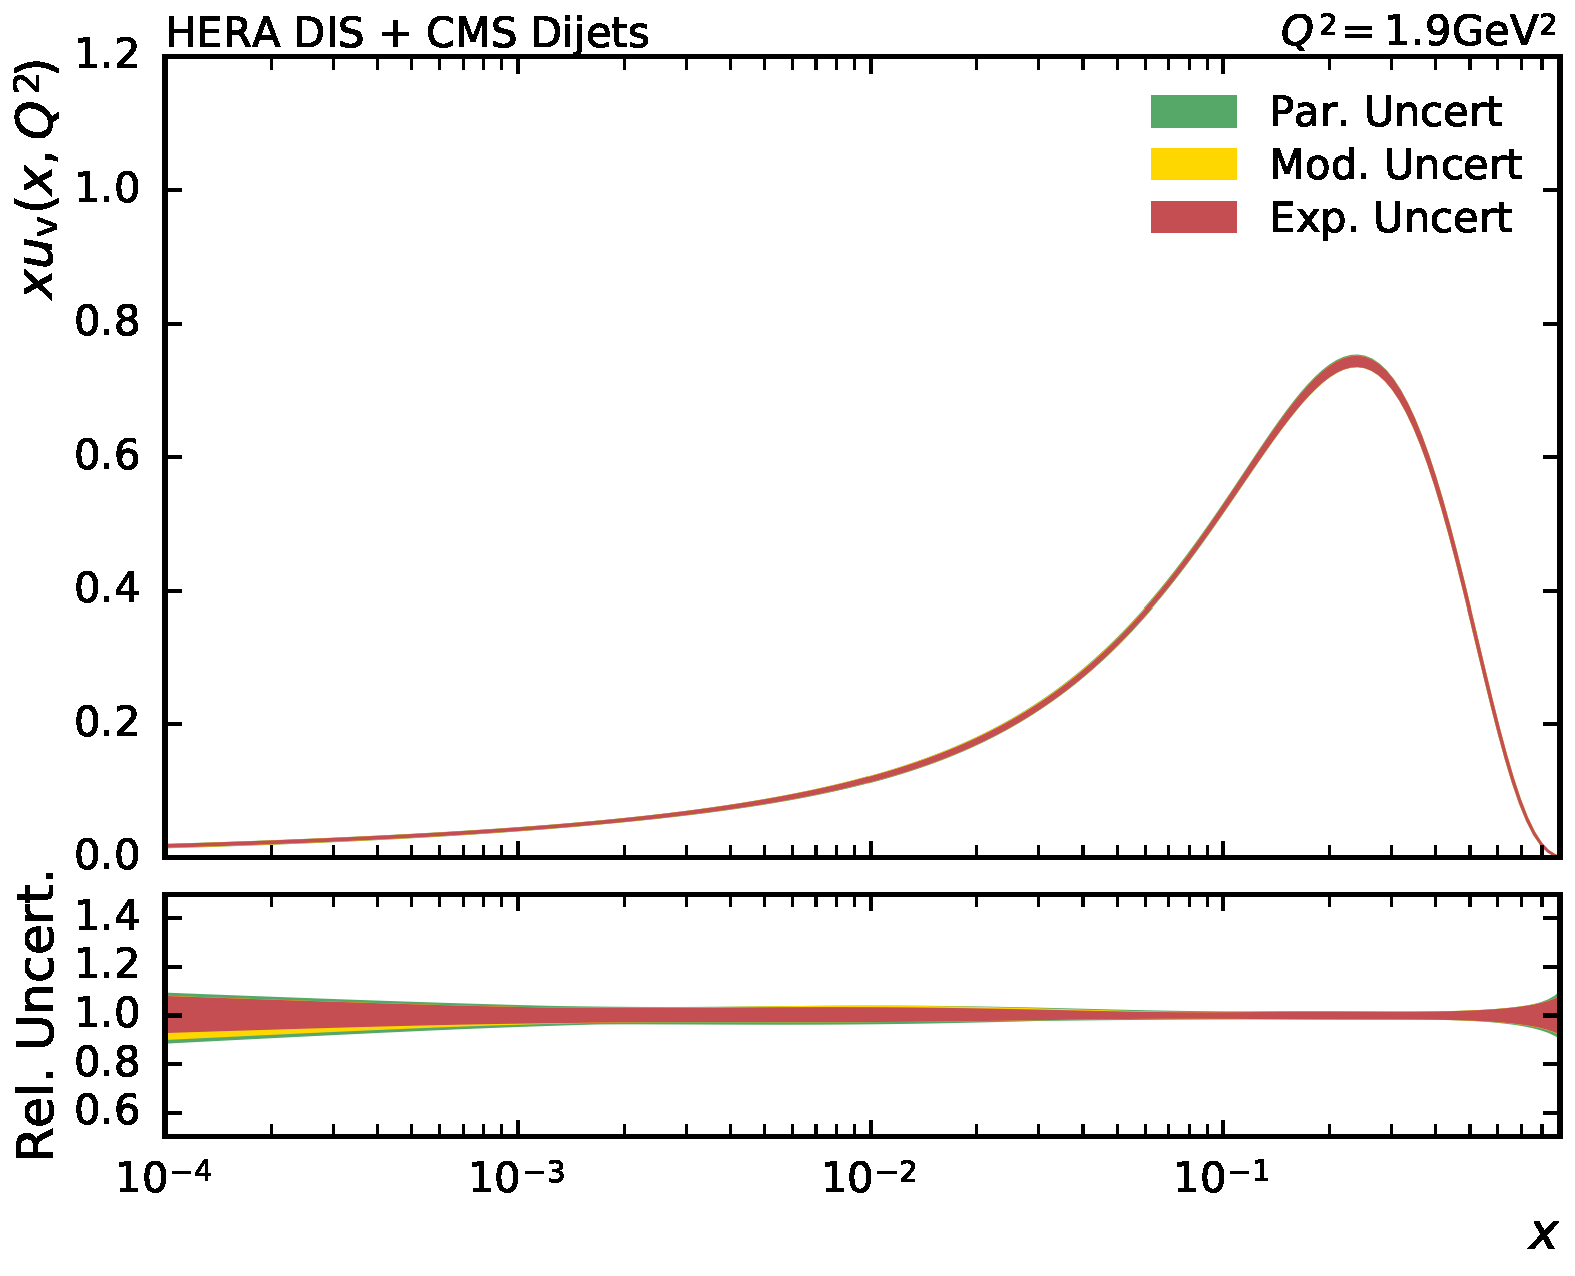
\includegraphics[width=0.48\textwidth]{figures/pdf_constraints/pdfcomp_HFTD_HERACMSTDJETS_8_1.9.pdf}

  \caption[The d valence and u valence quark PDFs]{The d valence quark (top) and u
    valence quark (bottom) PDFs as a function of $x$ as
  derived from HERA inclusive DIS data alone (left) and in combination with
  the CMS dijet data (right). The PDFs are shown at the starting scale $Q^2 =
  \SI{1.9}{\GeV \squared}$. The experimental (inner band), model (middle band)
  and parametrization uncertainties (outer band) are added quadratically to give
  the total uncertainty.}
  \label{fig:pdfconstraints:split:dvaluval:19}
\end{figure}

\begin{figure}[tbp]
  \centering
  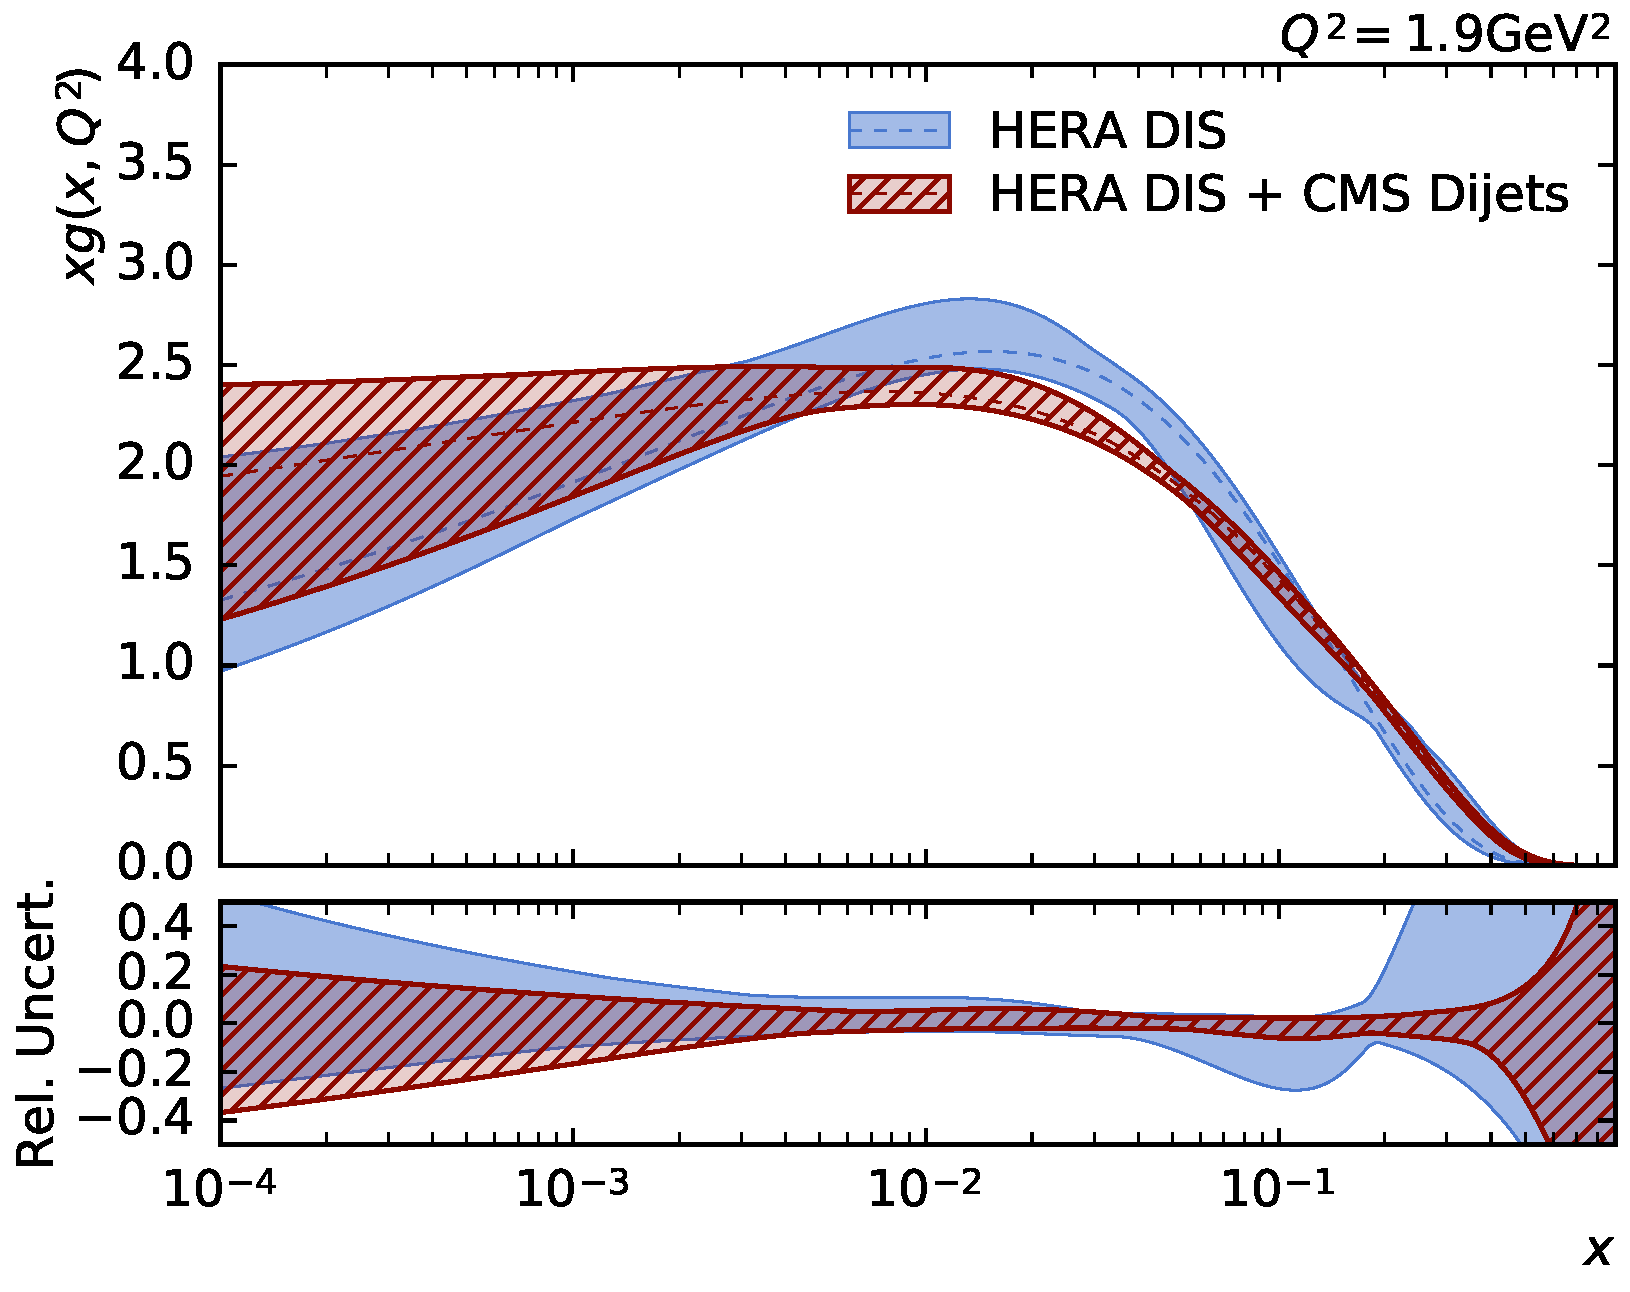
\includegraphics[width=0.48\textwidth]{figures/pdf_constraints/pdfcomp_direct_0_1.9.pdf}\hfill%
  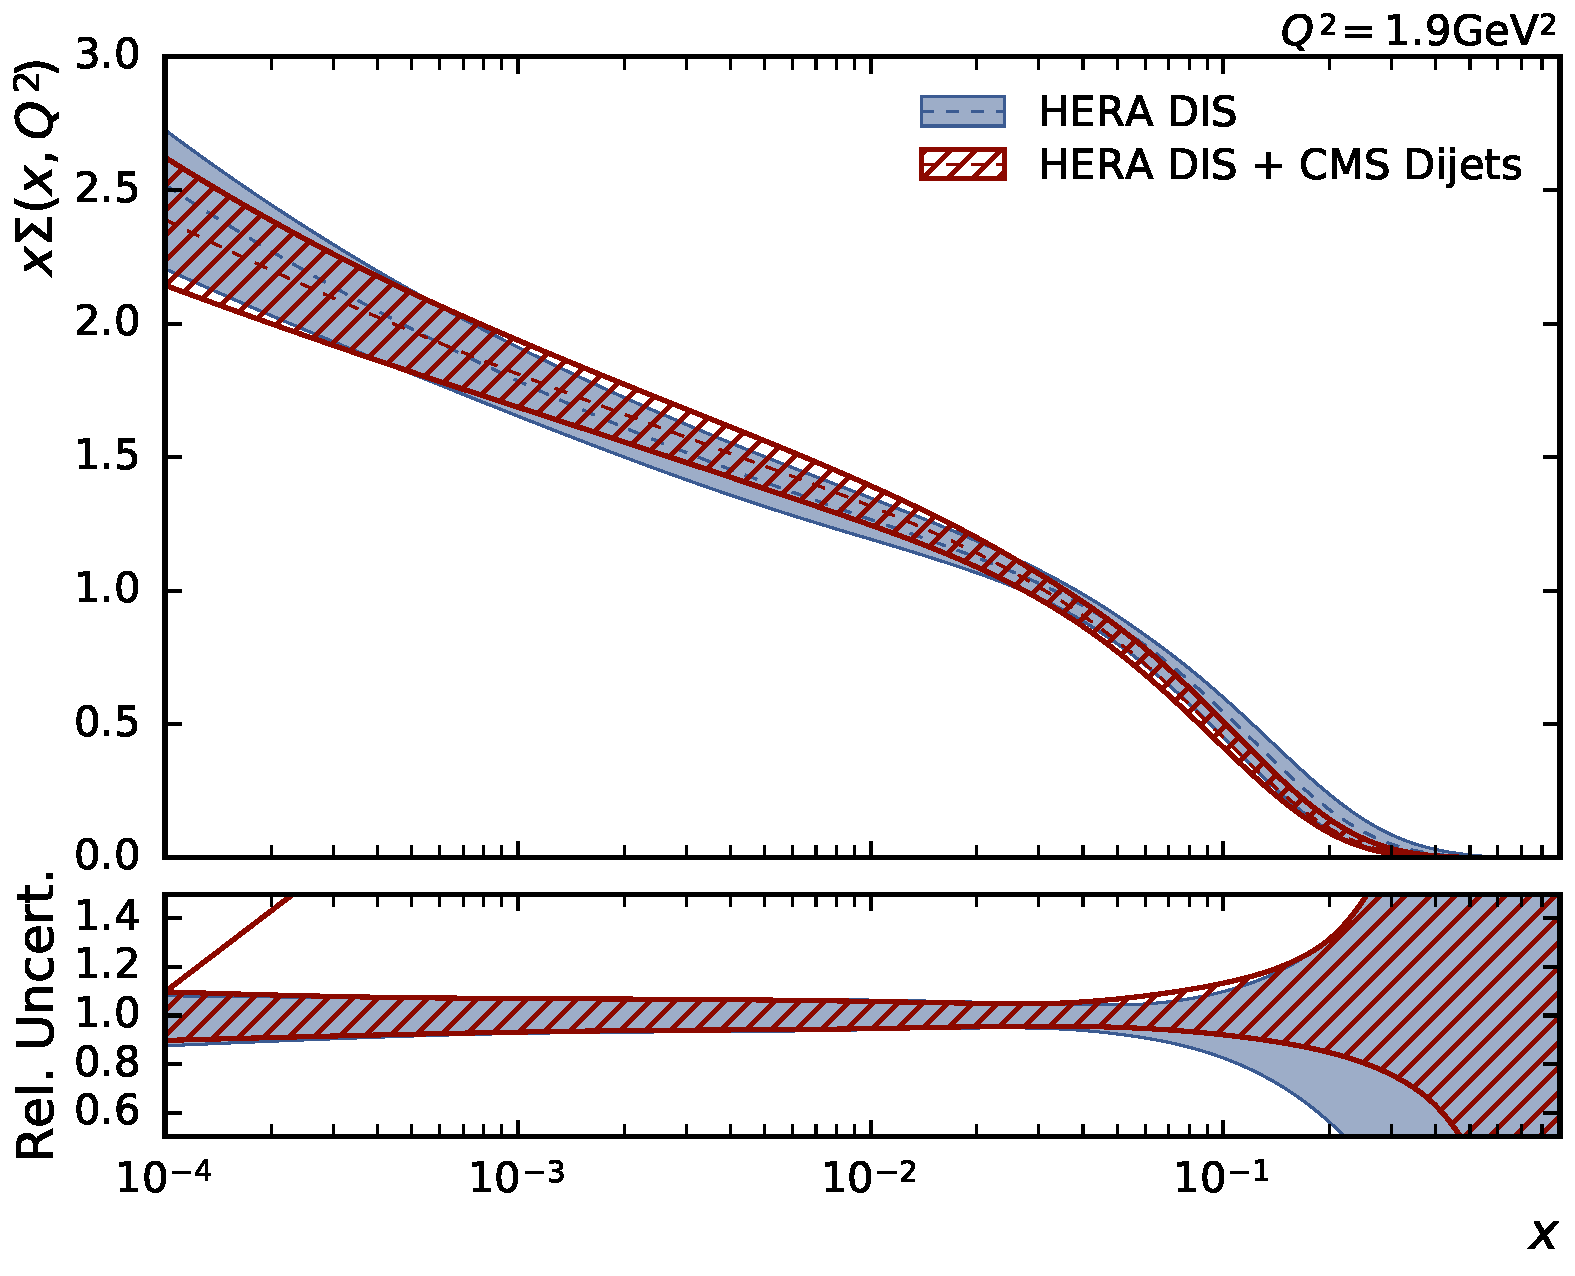
\includegraphics[width=0.48\textwidth]{figures/pdf_constraints/pdfcomp_direct_9_1.9.pdf}
  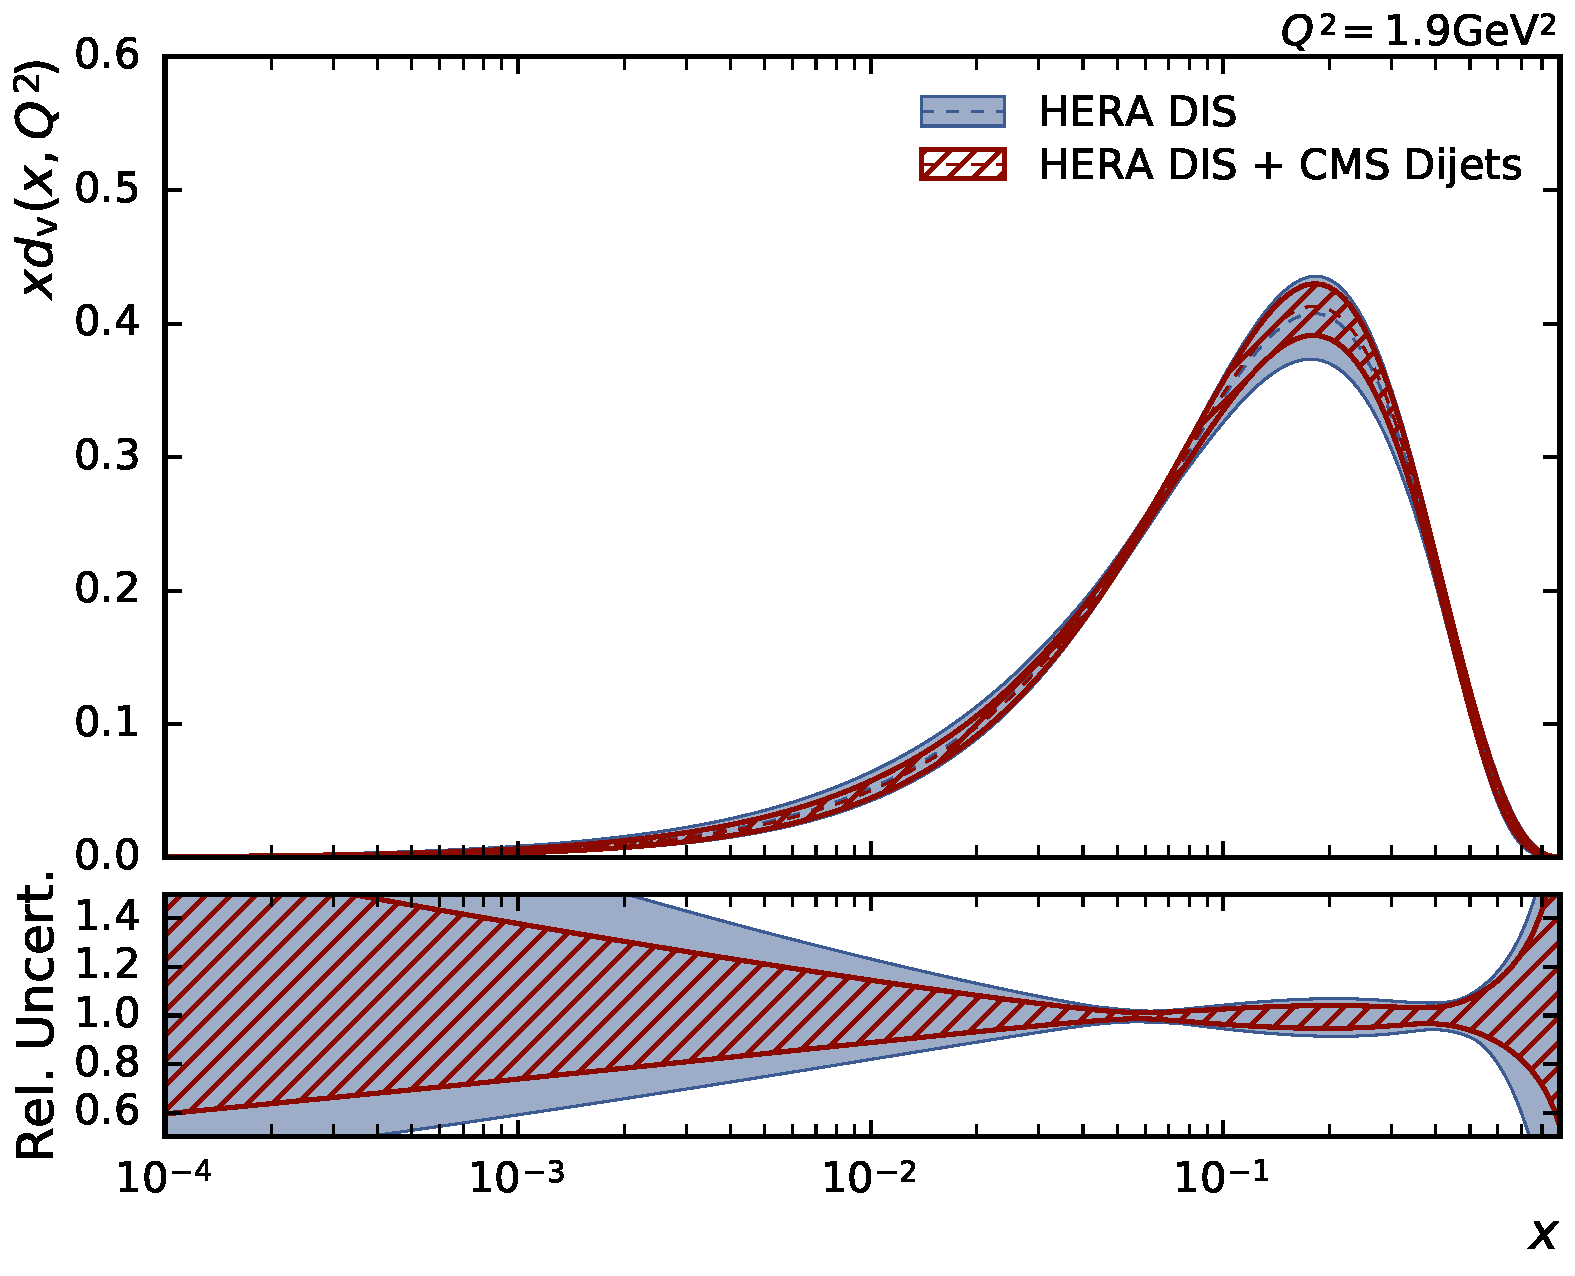
\includegraphics[width=0.48\textwidth]{figures/pdf_constraints/pdfcomp_direct_7_1.9.pdf}\hfill%
  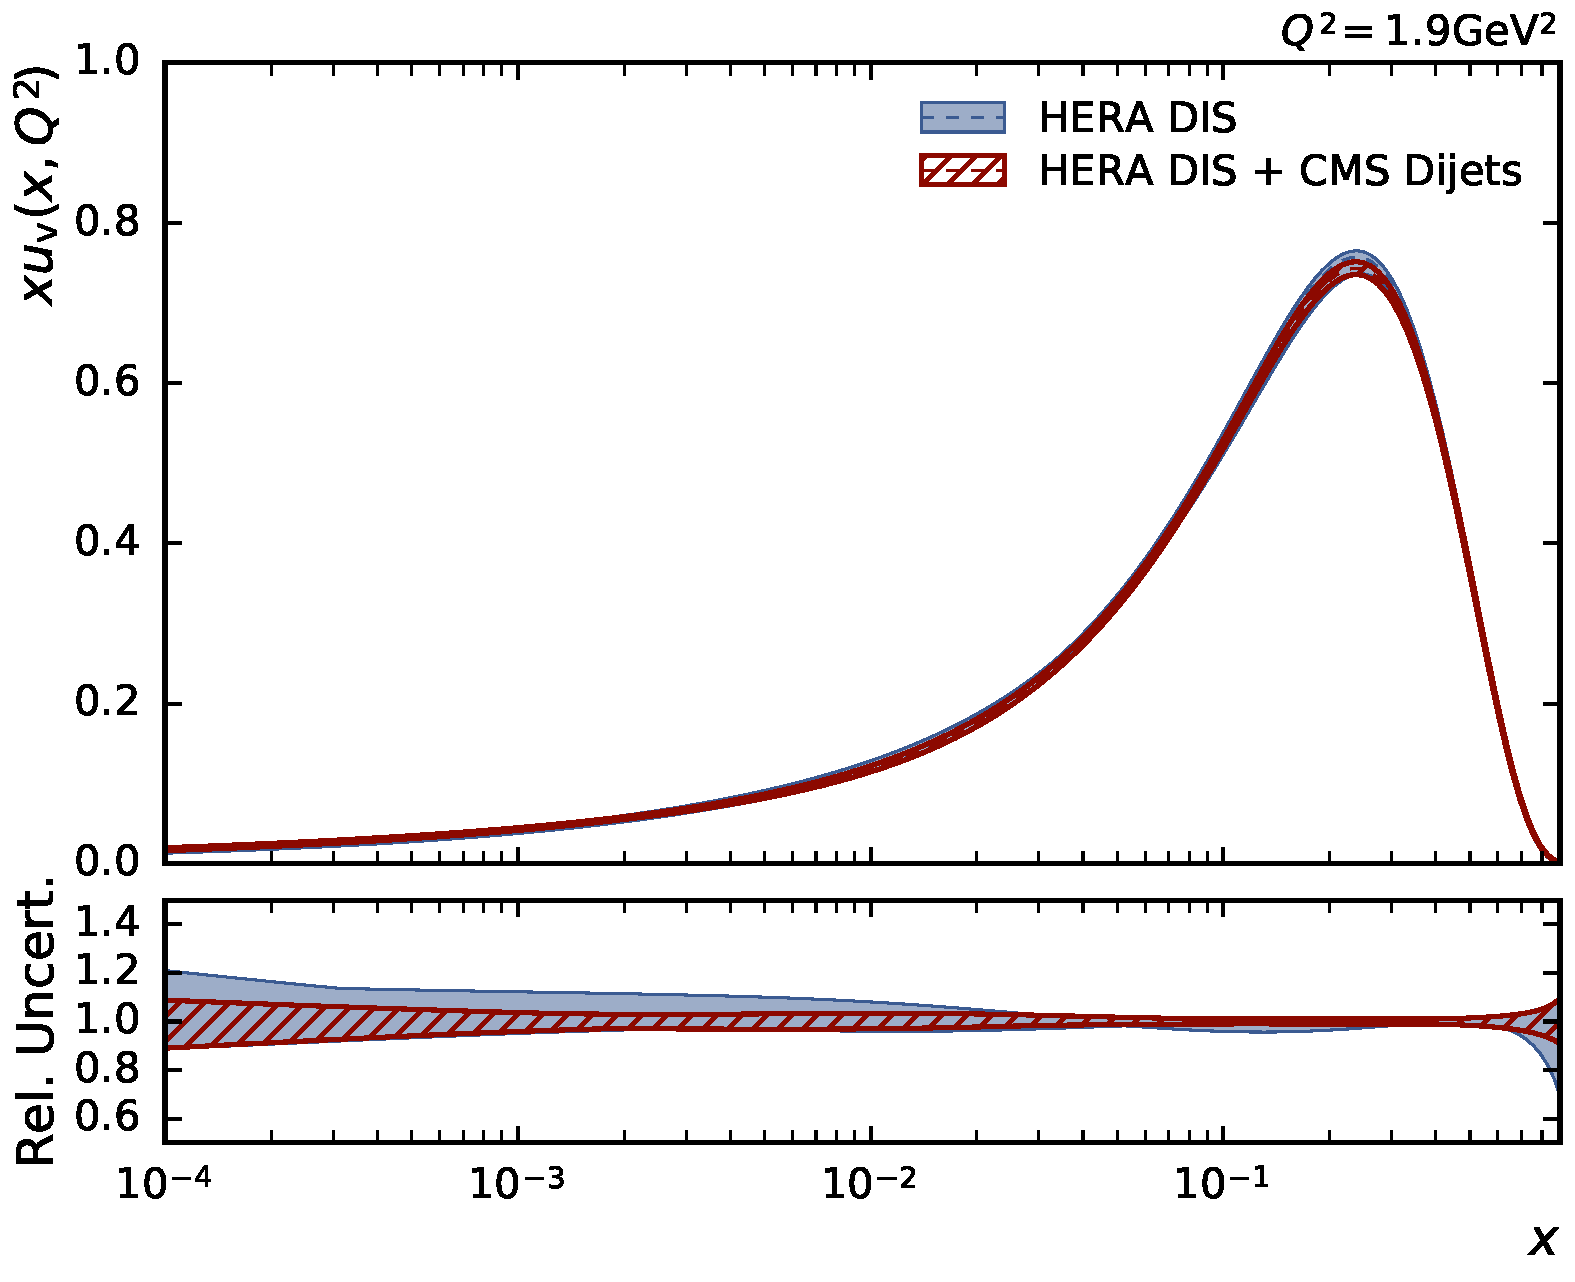
\includegraphics[width=0.48\textwidth]{figures/pdf_constraints/pdfcomp_direct_8_1.9.pdf}
  \caption[Direct comparison of gluon and quark PDFs]{The gluon (top left), sea
  quark (top right), d valence quark (bottom left) and u valence quark (bottom
right) PDFs as a function of $x$ as derived from HERA inclusive DIS data
alone (hatched band) and in combination with CMS dijet data (solid band). The PDFs
are shown at the starting scale $Q^2 = \SI{1.9}{\GeV \squared}$. The total
uncertainty of the PDFs is shown.}
  \label{fig:pdfconstraints:direct:19}
\end{figure}

\begin{figure}[tbp]
  \centering
  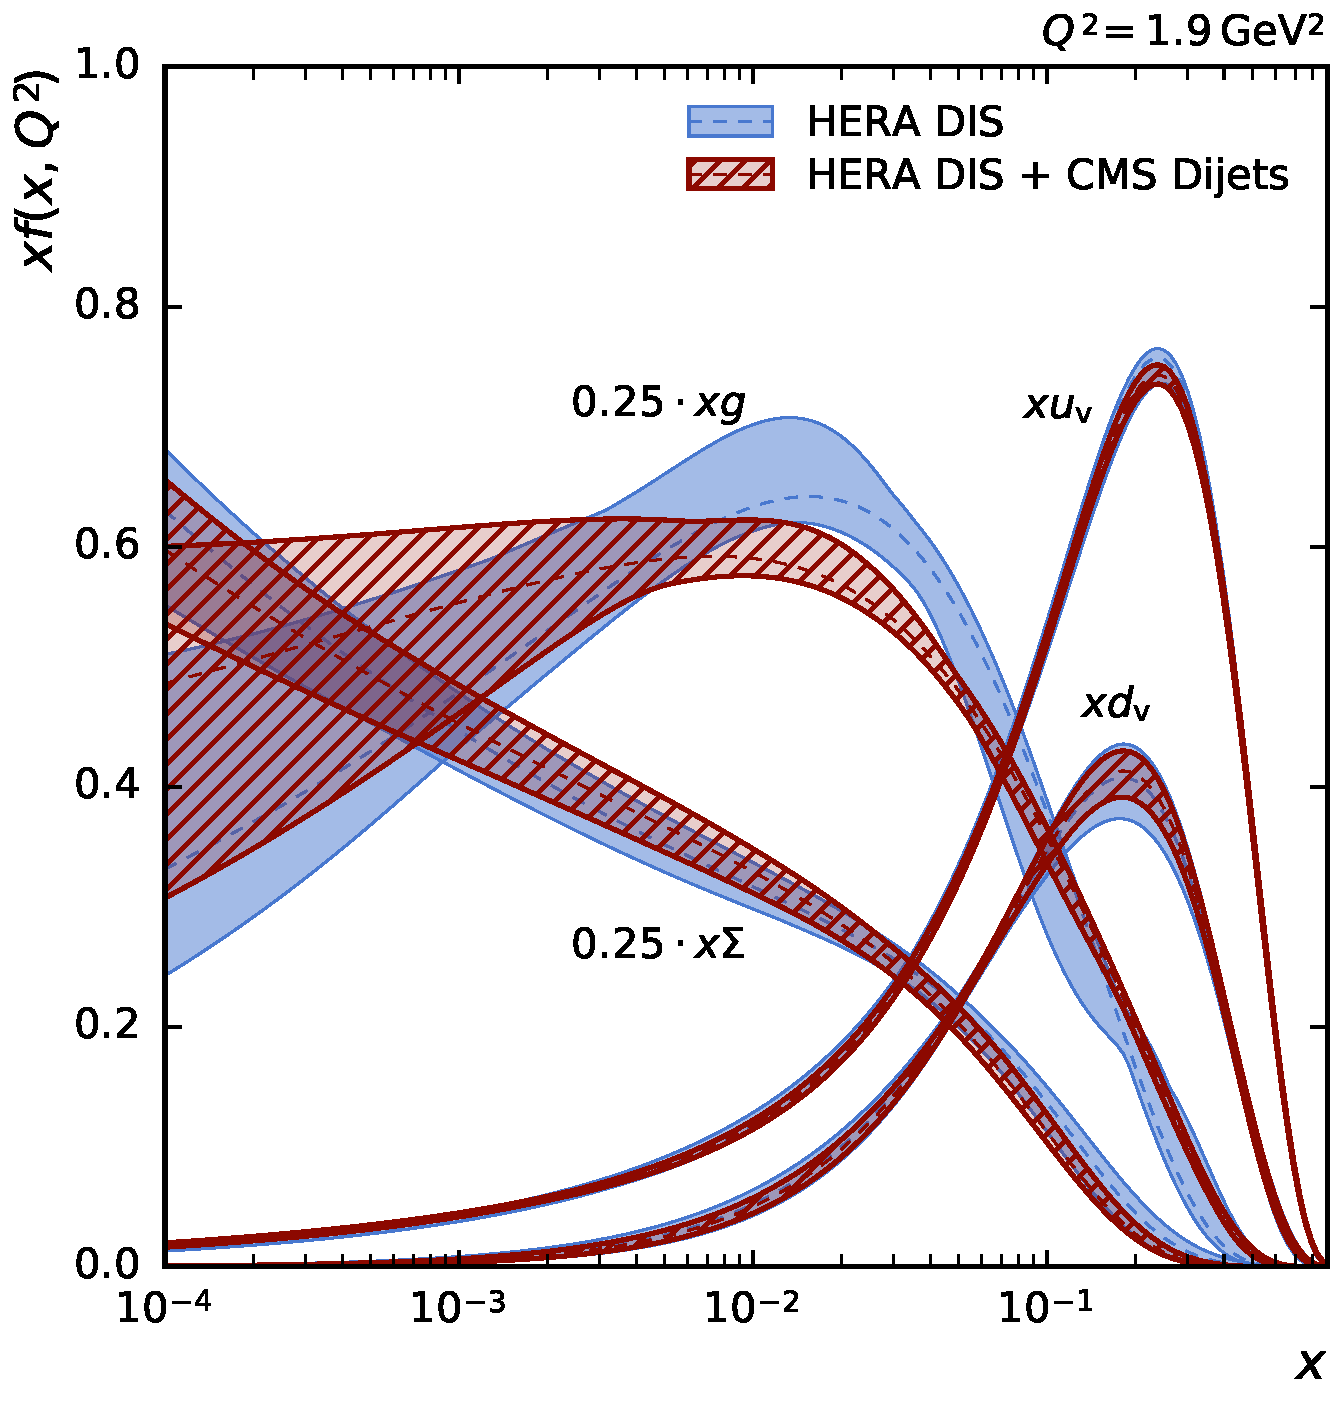
\includegraphics[width=0.7\textwidth]{figures/pdf_constraints/pdfcomp_direct_overview_1.9.pdf}\hfill%
  \caption[Overview of gluon and quark PDFs]{Overview of the gluon, sea, u
  valence and d valence quark PDFs before (hatched band) and after (solid band)
  including the CMS dijet data in the fit. The PDFs are shown at the starting
  scale $Q^2 = \SI{1.9}{\GeV \squared}$. The PDFs are shown with total
  uncertainties. The uncertainties of the PDF, especially of the gluon PDF, are
  significantly reduced. Moreover, a change of the gluon PDF shape is observed, resulting in a
  harder gluon after including the dijet data.}
  \label{fig:pdfconstraints:overview:19}
\end{figure}

\section{Simultaneous Fit of PDFs and Strong Coupling Constant}

The measurement of triple-differential dijet cross sections does not only
provide constraints on the PDFs, but also on the strong coupling constant. As
shown in the preceding part of the chapter, the region containing boosted dijet events is
the most sensitive regarding the PDFs. However, the \as sensitivity is higher in
the central bin in which highest transverse momenta are reached, and the
experimental uncertainties are smallest.

Due to the known correlation between the different phase space regions in this
measurement, this can be exploited by performing a fit of the PDFs and the
strong coupling simultaneously. Since the HERA DIS data are not that sensitive
to the \asmz value, a very consistent value of \asmz is extracted from the CMS
dijet data as no other data enter the fit. This is a major advantage of this
method. A disadvantage of such a fit is that unlike in a global PDF fit, further
constraints from other measurements on the PDFs are neglected. 

The fit is setup in exactly the same manner as
in the previous PDF studies. One additional free parameter is included, the
strong coupling constant \asmz. The obtained value for the strong coupling constant
reads
%
\begin{equation*}
  \asmz = 0.1194_{-0.0015}^{+0.0015}(\mathrm{exp})_{-0.0002}^{+0.0002}(\mathrm{mod})_{-0.0004}^{+0.0002}(\mathrm{par})
\end{equation*}
%
where the experimental uncertainty accounts for all sources of uncertainties of
the HERA and CMS data sets. NP uncertainties, which were also included in the
fit, are accounted for in the experimental uncertainty. However, the NP
uncertainties are comparably small and do not have a significant influence on the total
experimental uncertainty when added quadratically. Furthermore, model and parametrization uncertainties
were calculated in the same way as in the PDF determination. 

The consideration of scale uncertainties in a PDF fit is an open issue.
Therefore, two different methods to evaluate the scale uncertainty on \asmz were
studied. Similar to what is reported in Sec.~\ref{sec:scale_uncertainties}, the
renormalization and factorization scale were varied in the calculation of the
dijet data. The simultaneous fit was repeated for each variation. The envelope
of the best fit \asmz values for all variations is taken as uncertainty:
$\Delta\asmz= _{-0.0016}^{+0.0026}(\mathrm{scale})$.

The second procedure is analogous to the method which was applied in previous
determinations of \asmz \eg in~\cite{CMS:2014mna,Khachatryan:2014waa}. The PDFs
are derived for a series of fixed values of \asmz. Using this series, the best
fit \asmz value of the dijet data is determined for each scale variation. As
before, the envelope of all variations is taken as scale uncertainty: $\Delta
\asmz = _{-0.0019}^{+0.0031}(\mathrm{scale})$. Since this uncertainty is the
most consistent to compare with previous determinations of \asmz, it is reported
as the default one. 

The determined value of \asmz is in agreement with the world average of
$\asmz=0.1181\pm 0.0013$ determined by the PDG~\cite{Agashe:2014kda}.
